\documentclass[11pt]{article}
\usepackage[T1]{fontenc}
\usepackage{lmodern}
\usepackage[margin=1in]{geometry}
\usepackage{amsmath,amssymb,amsthm,mathtools}
\usepackage{microtype}
\usepackage{needspace}
\usepackage{enumitem,booktabs}
\usepackage{tikz}
\usetikzlibrary{arrows.meta,positioning}
\usepackage[colorlinks=true,linkcolor=blue,citecolor=blue,urlcolor=blue]{hyperref}
\usepackage[nameinlink,noabbrev]{cleveref}
\hypersetup{
 pdftitle={Memory and precision in noiseless Gaussian regression},
 pdfauthor={OpenAI},
 pdfsubject={Finite-state sample lower bounds for exact Gaussian observations},
 bookmarksopen=true,bookmarksnumbered=true,bookmarksopenlevel=1
}
\newtheorem{theorem}{Theorem}[section]
\newtheorem{proposition}[theorem]{Proposition}
\newtheorem{lemma}[theorem]{Lemma}
\newtheorem{corollary}[theorem]{Corollary}
\newtheorem{claim}[theorem]{Claim}
\theoremstyle{definition}
\newtheorem{definition}[theorem]{Definition}
\theoremstyle{remark}
\newtheorem{remark}[theorem]{Remark}
\newcommand{\R}{\mathbb R}
\newcommand{\N}{\mathbb N}
\newcommand{\E}{\mathbb E}
\newcommand{\Prob}{\mathbb P}
\newcommand{\sphere}{S^{d-1}}
\newcommand{\norm}[1]{\left\lVert #1\right\rVert}
\newcommand{\ip}[2]{\langle #1,#2\rangle}
\newcommand{\ind}{\mathbf 1}
\newcommand{\dist}{\operatorname{dist}}
\newcommand{\supp}{\operatorname{supp}}
\newcommand{\aff}{\operatorname{aff}}
\newcommand{\vol}{\operatorname{vol}}
\newcommand{\op}{\mathrm{op}}
\DeclareMathOperator{\rank}{rank}

\title{Memory and precision in noiseless Gaussian regression}
\author{OpenAI}
\date{September 27, 2026}
\begin{document}
\maketitle
\begin{abstract}
For every fixed \(A>0\), a learner that retains at most \(Ad^2\) bits
between fresh exact Gaussian linear measurements needs
\(\Omega_A(d\log(1/\epsilon))\) measurements to estimate a uniformly
random unit vector to angular error at most \(\epsilon\), for any
\(0<\epsilon\le 1/10\), with probability at least \(2/3\). The constant
is absolute for \(o(d^2)\) memory.
\end{abstract}
\tableofcontents
\section{Exact observations and finite memory}\label{h:introduction}

An exact linear equation carries arbitrarily fine information. Indeed,
\(d\) independent Gaussian equations determine an unknown vector in
\(\R^d\) almost surely if all the equations can be retained. A learner
that reads the equations once and remembers only a finite state faces
a different problem. Increasing the required accuracy can force it to
read more equations even when every equation is noiseless.

\begin{definition}[Finite-state Gaussian regression]\label{h:model}
Fix integers \(d\ge2\), \(M\ge0\), and \(T\ge0\). A data-independent
shared seed may choose the learner's rules; the descriptions of its
transitions and output below are conditional on that seed. A signal
\(s\in S^{d-1}\) is chosen before sampling. At sample index
\(t\in\{1,\ldots,T\}\), the observation is
\[
 x_t\sim N(0,I_d),\qquad y_t=\ip{x_t}{s},
\]
where the rows \(x_1,\ldots,x_T\) are independent. A learner reads the
pairs once, in order. After each number of samples its persistent state
belongs to a prescribed set of at most \(2^M\) elements. The initial
state and shared seed are jointly independent of the signal and all
rows, but may depend on each other. Conditional on the seed and state,
a transition may use the entire current pair and fresh
randomness, with unrestricted computation, but only the next finite
state is retained.

The learner may stop, including before the first sample, but must stop
by the prescribed deterministic finite horizon \(T\). At a stopping index its unit
output \(\widehat s\in S^{d-1}\) is generated from the terminal state,
the stopping index, and fresh randomness only. In particular, a
discarded observation cannot be read again by the output rule.
The transitions and stopping rules may depend on \(d\), the requested
accuracy \(\epsilon\), and the index, but not on \(s\).

The experiment must be jointly measurable in the signal, the complete
pre-generated rows, the shared seed, the initial state, and all fresh
transition and output randomness. Conditional on the seed, each fixed
state/index transition and stopping probability must be Borel in
\((x,y)\), or measurable in the completion of
\(\lambda_1(dx,dy)=\gamma_1(dx)\,dy\), where \(\gamma_1\) is standard
Gaussian probability on \(\R^d\). Fresh randomness supplies no
information about the signal or samples beyond the permitted rule
arguments. Accuracy means
\[
 \arccos\ip{\widehat s}{s}\le\epsilon.
\]
\end{definition}

The state bound measures bits, not real registers. The rules can be
nonuniform in the dimension and sample index, and randomization is
allowed both in choosing the rules and during the run. The model fixes
the rows in advance through their independent Gaussian law: it does
not allow a learner to choose a row or revisit an earlier one.

Write \(\sigma_d\) for uniform probability on \(S^{d-1}\). Our main
statement assumes success only after averaging over this prior.

\begin{theorem}[Memory and precision]\label{h:main}
For every fixed finite \(A>0\), there are constants \(c_A>0\) and
\(d_A\) such that the following holds. Let \(d\ge d_A\), let
\(0\le M\le Ad^2\) be an integer, and let \(0<\epsilon\le1/10\).
For any learner in Definition~\ref{h:model}, draw
\(S\sim\sigma_d\) independently of the rows and the learner's
data-independent randomness. If
\[
 \Prob\{\arccos\ip{\widehat s}{S}\le\epsilon\}\ge\frac23,
\]
then its prescribed horizon satisfies
\[
 T\ge c_A\,d\log(1/\epsilon).
\]
\end{theorem}

Here and throughout the paper logarithms are natural unless a base is
shown. The constants in Theorem~\ref{h:main} may depend on the fixed
number \(A\). The statement makes no uniform claim when \(A=A(d)\)
tends to infinity. No relation between \(\epsilon\) and \(M\) is
assumed.

\begin{corollary}[Subquadratic memory]\label{h:subquadratic}
Let \(M(d)\ge0\) be integer-valued with \(M(d)=o(d^2)\), and let
\(0<\epsilon(d)\le1/10\) be any accuracy sequence. A family of learners
in Definition~\ref{h:model} with uniform-sphere average success at
least \(2/3\) satisfies
\[
 T(d)\ge c\,d\log(1/\epsilon(d))
\]
for all sufficiently large \(d\), where \(c>0\) is absolute. The
dimension threshold may depend on the memory sequence.
\end{corollary}

\begin{corollary}[A guarantee for every signal]\label{h:worst-signal}
The conclusions of Theorem~\ref{h:main} and
Corollary~\ref{h:subquadratic} also hold when their average-success
assumption is replaced by
\[
 \Prob\{\arccos\ip{\widehat s}{s}\le\epsilon\}\ge\frac23
 \qquad\text{for every }s\in S^{d-1},
\]
where this probability is over the rows and the learner's randomness.
\end{corollary}

The every-signal consequence follows by averaging the same learner
over \(\sigma_d\); it does not say that every individual signal is hard
for every learner. We prove Theorem~\ref{h:main} and both corollaries
after completing the backward argument in Section~\ref{h:end:section}.

\paragraph{The original experiment and measurable versions.}
All success probabilities refer to the original jointly measurable
experiment. Joint independence of the initial state and seed from the
signal and rows permits conditioning on the seed without changing the
prior or supplying information through initialization.
Section~\ref{h:stream:section} replaces completed-measurable rules
by Borel versions separately for almost every seed, preserving the
corresponding prior success probabilities. Their average is taken
in the original experiment; no jointly measurable choice of all these
versions is assumed.

\subsection{The precision problem and its predecessors}

Memory constraints in statistical learning were studied before this
precision question. Shamir's finite-message framework included
bounded-memory online processing as a special case
\cite[Section~2, Definition~1]{Shamir2014}. In its general form a
protocol may retain an entire transcript, so its per-message budget is
not a bound on total persistent memory. Steinhardt and Duchi proved
memory-dependent minimax risk bounds for sparse noisy regression
\cite[Section~1.1, Equation~(2)]{SteinhardtDuchi2015}. Their hard
family uses positive noise and a different covariate distribution.
These works established that information retained from earlier samples
can be a statistical resource in its own right.

Steinhardt, Valiant, and Wager connected memory, communication, and
statistical queries, and formulated a quadratic-memory versus
exponential-sample question for parity learning
\cite[Section~1.1, Conjecture~1]{SVW2016}. Raz proved the qualitative
separation for parity \cite[Theorem~1 and Remark~1.1]{Raz2016} and
developed a spectral method for a wider class of learning problems
\cite{Raz2017}. The qualifier \emph{qualitative} matters: Raz's
theorem and the published conjecture have different numerical
memory coefficients. These discrete results explain the usefulness of
finite-width computation models, but they do not supply an estimate
for exact real-valued observations.

Among the sources discussed here, the closest continuous-regression
comparison is due to Sharan, Sidford, and Valiant
\cite{SSV2019}. Their Theorem~1 uses independent \(N(0,I_d)\)
covariates, a fixed unit target, and independent uniform additive noise
of half-width \(2^{-d/5}\). With at most \(d^2/4\) bits and Euclidean
accuracy \(\epsilon=d^{-r}\), it gives an
\(\Omega(d\log r)\) sample lower bound for \(r\) from a sufficiently
large absolute constant up to order \(d/\log d\), in the range stated
there. Their proof experiment draws the target uniformly on the sphere
and averages over it and the samples \cite[Section~2]{SSV2019}.
Their nonuniform finite-width layered program is a predecessor of the
model above; the measurable randomized rules and bounded stopping used
here are handled directly in Section~\ref{h:stream:section}.

The observation law is the important difference. A lower bound with
additive noise does not by itself bound the more informative exact
experiment. Theorem~\ref{h:main} treats the exact-observation precision
question for isotropic Gaussian rows. Section~1.1 of \cite{SSV2019}
asks whether the first-order sample dependence on precision is optimal
under bounded memory. This is distinct from its separate
condition-number conjecture for ill-conditioned Gaussian laws and
constant Euclidean accuracy in \cite[Section~1.1]{SSV2019}.

Dagan, Kur, and Shamir obtained related quadratic-space obstructions
for two other linear-prediction tasks \cite{DKS2019}. Their published
Theorem~3 asks for a unit approximate null vector of independent
Gaussian rows. Their Theorem~10 asks for small empirical residual on
a finite random-order system built from jointly conditioned sphere
rows and one fixed equation. These are different targets and
observation laws from the fixed-signal stream considered here.

\paragraph{A consequence for the noisy experiment.}
Theorem~\ref{h:main} implies an
\(\Omega_A(d r\log d)\) sample lower bound in the noisy Gaussian
experiment of Sharan, Sidford, and Valiant \cite{SSV2019}, for every
fixed finite \(A>0\), memory \(M\le Ad^2\), and Euclidean accuracy
\(e=d^{-r}\) in their fine-accuracy range described above,
for sufficiently large \(d\). Here success is at least \(2/3\)
averaged over the uniform-sphere target, and learners retain the state,
deterministic-horizon, randomness, and joint and per-seed measurability
conventions of Definition~\ref{h:model}, with a terminal estimate
\(V\in\R^d\) depending only on the terminal state, stopping index,
and fresh randomness. An exact-observation learner generates the
prescribed independent uniform noise inside each current-pair
transition and simulates the noisy learner with the same states and
horizon. For completed rules, the noisy pair law has a density with
respect to \(\lambda_1\), so the Borel-version and seed-conditioning
argument of Section~\ref{h:stream:section} applies before this
simulation. On \(\|V-S\|\le e\le1/20\), normalizing \(V\) gives
angular error at most \(\arcsin e\le2e\); assign any unit output when
\(V=0\). Theorem~\ref{h:main} at accuracy \(2e\) therefore gives
\(T\ge c_A d\log(1/(2e))=\Omega_A(d r\log d)\).

\subsection{Why the precision scale is natural}

With real registers, the classical Kaczmarz projection step
\cite{Kaczmarz1937}, in the form stated by Strohmer and Vershynin
\cite[Algorithm~1]{SV2009}, gives a simple benchmark. Starting with
\(z_0=0\), use
\begin{equation}\label{h:kaczmarz}
 z_t=z_{t-1}+
 \frac{y_t-\ip{x_t}{z_{t-1}}}{\norm{x_t}^2}\,x_t
 \qquad(x_t\ne0),
\end{equation}
and set \(z_t=z_{t-1}\) on the Gaussian-null event \(x_t=0\).
For \(u_t=x_t/\|x_t\|\), the error is multiplied by
\(I-u_tu_t^{\mathsf T}\). The direction \(u_t\) is fresh and uniform
on the sphere, so \(\E(u_tu_t^{\mathsf T})=I_d/d\). Conditional on
the previous error,
\[
 \E\!\left(\norm{z_t-s}^2\mid z_{t-1}\right)
  =(1-1/d)\norm{z_{t-1}-s}^2.
\]
Induction gives
\begin{equation}\label{h:kaczmarz-contraction}
 \E\norm{z_t-s}^2=(1-1/d)^t.
\end{equation}
This calculation explains the scale \(d\log(1/\epsilon)\) for fresh
isotropic observations. Strohmer and Vershynin's theorem concerns
norm-weighted sampling from a fixed finite matrix; the equality above
is the separate symmetry calculation for this stream. The displayed
update stores real scalars and supplies no finite-bit upper bound.

\subsection{A backward proof under the original prior}

Conditioning the uniform prior on one raw exact observation almost
surely confines the signal to a hyperplane section of the sphere. That
conditional law is singular relative to the original spherical
measure. We instead keep the original prior fixed and study the
probability of future success from a prescribed state.

Start the learner at a chosen state and index, whether or not the state
was reached in an actual run. Let \(h(s)\) be its success probability
with signal \(s\), using fresh future samples. For a closed Euclidean
ball \(B(z,r)\), our invariant is
\begin{equation}\label{h:intro:invariant}
 \int_{B(z,r)}h\,d\sigma_d\le(Rr)^{(d-1)/2}
 \qquad(z\in S^{d-1},\ r>0).
\end{equation}
The number \(R\) bounds the concentration of successful signals; it
is not a radius supporting a posterior. A terminal output rule has
\(R=\epsilon\). Moving backward across a block of order \(d\)
observations multiplies \(R\) by at most a constant for fixed
\(M/d^2\). Constant average success requires \(R\) bounded below, so
reaching it from \(\epsilon\) takes order \(\log(1/\epsilon)\) blocks.

The bound at every radius makes this iteration close. Restrict
\(h\,d\sigma_d\) to a ball \(B(z,r)\), without conditioning on reaching
a state or dividing by the restricted mass. This finite measure has
an ambient ball bound \(H t^\beta\), with \(\beta=(d-1)/2\) and
\(H\) controlled by \(R^\beta\). The general projection estimate in
Section~\ref{h:projection} gives the joint law of a Gaussian matrix
and its exact labels an \(L^q\) density whose norm is bounded by
\[
 e^{Cd}H r^{\beta-m(1-1/q)}
\]
for a block of \(m\le q\) rows, where \(q\) is proportional to \(d\).
The density loses a radius power. The volume of the common projected
ellipsoid is at most \(e^{Cd}r^m\), and its power \(1-1/q\) restores
exactly that loss in H\"older's inequality.

The geometric step controls inverse distances to affine spans, hence
an inverse Gram determinant. Local growth and inverse-distance
averaging belong to the classical projection methods represented by
Mattila \cite[Lemma~5.1 and Theorem~5.4]{Mattila1975}; the
independent-copy expansion and successive orthogonalization have a
closer regression predecessor in
\cite[Section~7, Lemma~12]{SSV2019}. We derive the exact multirow
density and its quantitative bounds here. Its finite-measure
formulation does not require a density relative to spherical area.

Section~\ref{h:blocks} combines the projection and volume bounds
with a second application of H\"older on the \(N\) possible
destinations. Selection costs \(N^{1/q}\), so taking the
\((d-1)/2\)-th root in \eqref{h:intro:invariant} gives the memory
contribution \(\exp(O(\log N/d^2))\).
Section~\ref{h:stream:section} constructs fresh continuation
functions, counts only stopping indices within one block, and passes
from Borel rules to the full randomized model. Reflection across the
span of the observed rows gives the independent constant-accuracy
endpoint in Section~\ref{h:end:section}, completing the theorem.

The general projection estimate also applies to a lower-dimensional
cube prior on the sphere. That application has its own distributional
precision bound; the conclusion throughout the stated accuracy range
uses an every-signal guarantee and the separate uniform-sphere
endpoint. The appendices give distinct exact-label interfaces,
compare coefficient normalizations through one backward bound,
and retain a sharper full-data residual estimate.

\section{Local mass of terminal success}\label{h:local}

At a terminal state, the output law is independent of the unknown
signal. A small spherical ball has small uniform mass, and the same is
true of the set of signals close to a fixed output. Combining these
two facts initializes the bound that will be propagated backward.

Write \(\sigma=\sigma_d\), and let \(B(z,r)\) denote a closed
Euclidean ball in the ambient space of its center. Vector norms are
Euclidean, and \(\|A\|_{\op}\) is the Euclidean operator norm. Constants
denoted by \(C\) are positive and absolute and may increase between
displays. For the main proof set
\begin{equation}\label{h:local:parameters}
 n=d-1,\qquad a=\frac n2,\qquad
 q=\left\lfloor\frac n8\right\rfloor.
\end{equation}
We work in sufficiently large dimension that
\(q\ge2\), \(q\ge d/16\), and \(a\ge d/3\). These are absolute
dimension requirements. The real number \(a\) is a local-mass
exponent, whereas the integer \(q\) is a projection-moment order.

For \(R>0\), say that a measurable \(h:S^{d-1}\to[0,1]\) has local
mass at scale \(R\) if
\begin{equation}\label{h:local:bound}
 \int_{B(z,r)}h\,d\sigma\le(Rr)^a
 \qquad(z\in S^{d-1},\ r>0).
\end{equation}
The scale is an upper-bound parameter; it is not a support radius.

\begin{lemma}[Spherical balls and terminal outputs]\label{h:local:caps}
For \(d\ge2\), \(z\in S^{d-1}\), and \(r>0\),
\begin{equation}\label{h:local:cap}
 \sigma_d(B(z,r))\le r^{d-1}.
\end{equation}
Consequently, if \(Q\) is any probability law on \(S^{d-1}\)
independent of the signal and
\[
 h(s)=Q\{v:\arccos\ip{v}{s}\le\epsilon\},
\]
then \(h\) has local mass at scale \(R=\epsilon\):
\begin{equation}\label{h:local:terminal}
 \int_{B(z,r)}h\,d\sigma_d\le(\epsilon r)^{(d-1)/2}.
\end{equation}
\end{lemma}

\begin{proof}
For \(0<r\le1\), rotate \(z\) to the north pole and write
\(n=d-1\). A point of \(S^{d-1}\cap B(z,r)\) has last coordinate at
least \(1-r^2/2\ge1/2\). On the upper hemisphere the surface-area
element as a graph over the first \(n\) coordinates is the reciprocal
of that last coordinate, hence at most two on this cap. Its projection
is contained in the \(n\)-ball of radius \(r\). The full sphere has
area at least twice the volume of the unit \(n\)-ball, since both
hemispheres project onto that ball with area element at least one.
The ratio is at most \(r^n\). For \(r>1\), the total mass one gives
the same inequality.

If the angular distance from a fixed unit output \(v\) is at most
\(\epsilon\), its chordal distance is
\(2\sin(\theta/2)\le\theta\le\epsilon\). Thus the global successful
mass for \(v\) is at most \(\epsilon^n\). Integrating this inequality
against \(Q\) gives the same global bound for \(h\). Independently,
\(0\le h\le1\) and \eqref{h:local:cap} give local mass at most \(r^n\).
Therefore
\[
 \int_{B(z,r)}h\,d\sigma_d
 \le\min\{r^n,\epsilon^n\}\le(\epsilon r)^{n/2},
\]
where the last inequality follows by considering \(r\le\epsilon\)
and \(r\ge\epsilon\).
\end{proof}

The two bounds play different roles: \(r^{d-1}\) controls
concentration in a small region, and \(\epsilon^{d-1}\) controls the
total successful mass. Their geometric mean has the same exponent in
\(r\) and \(\epsilon\), which is the form preserved by one block.

\section{Exact Gaussian projection}\label{h:projection}

A block of exact equations acts on a localized part of each
continuation's successful mass. We prove its projection bound for an
arbitrary finite measure with controlled mass in every ambient ball.
Keeping the coefficient and support radius visible will expose the
cancellation in the block estimate. The same theorem will later apply
to a prior supported on a lower-dimensional part of the sphere.

For a positive integer \(m\), let \(\gamma_m\) be the law of an
\(m\)-by-\(d\) matrix with independent standard Gaussian entries, and set
\[
 \lambda_m(dA,dy)=\gamma_m(dA)\,dy.
\]
For a finite nonnegative Borel measure \(\mu\), let \(\eta_\mu\) be
the image of \(\gamma_m(dA)\mu(ds)\) under
\((A,s)\mapsto(A,As)\). The matrix remains part of the observed data;
no normalization of \(\mu\) is made. The integer \(m\) counts rows,
while \(p\) below is a density moment order. Write \(v_m\) for the unit
\(m\)-ball volume. For a closed support ball \(B(z,R)\), define
\begin{equation}\label{h:dv:support-sets}
 \mathcal E_{z,R}=\{(A,y):y\in Az+A B(0,R)\}
 \subseteq
 \mathcal S_{z,R}
 =\{(A,y):\|y-Az\|\le R\|A\|_{\mathrm{op}}\}.
\end{equation}
The exact image is carried by \(\mathcal E_{z,R}\). This set is
Borel: it is the zero set of the continuous function
\((A,y)\mapsto\min_{\|v\|\le R}\|y-Az-Av\|\).
Changing \((A,y)\) changes this minimum by at most
\(\|y-y'\|+\|A-A'\|_{\mathrm{op}}(\|z\|+R)\).

In this section \(H\) is a local-mass coefficient and \(R\) is the
geometric radius of a supporting ball. This use of \(R\) is separate
from the propagated scale in \eqref{h:local:bound}.

\begin{theorem}[Exact projection density from an ambient ball bound]
\label{h:dv:finite-density}
Let \(d,m\ge1\) and \(p\ge2\) be integers, and let
\(\beta>m+p-2\), \(H,R>0\), and \(z\in\mathbb R^d\).
Suppose that \(\mu\) is a finite nonnegative Borel measure supported
on \(B(z,R)\) and satisfying
\begin{equation}\label{h:dv:ambient-bound}
 \mu(B(x,r))\le Hr^\beta
 \qquad(x\in\mathbb R^d,\ r>0).
\end{equation}
For \(0\le j\le p-2\), put
\[
 J_j=1+3^j2^\beta\frac{m}{\beta-j-m},
\]
and define
\begin{equation}\label{h:dv:moment-scale}
 \mathcal B=(2\pi)^{-m(p-1)/(2p)}
 H R^{\beta-m(1-1/p)}
 \left(\prod_{j=0}^{p-2}J_j\right)^{1/p}.
\end{equation}
Then \(\eta_\mu\) has a nonnegative jointly Borel density \(F\)
with respect to \(\lambda_m\), which can be chosen to vanish
outside \(\mathcal E_{z,R}\), and
\begin{equation}\label{h:dv:finite-density-bound}
 \|F\|_{L^p(\lambda_m)}\le\mathcal B.
\end{equation}
\end{theorem}

Projection loses \(m(1-1/p)\) powers of the support radius.
The volume of the projected ball will restore exactly this power.
We prove the theorem by controlling inverse affine distances,
expanding a smoothed density moment, and then removing the smoothing
on matrix--label space. The independent-copy moment and successive
orthogonalization have a close predecessor in the noisy regression
analysis of \cite[Section~7, Lemma~12]{SSV2019}. That result treats a
one-row noisy interval under a global \(L^2\) density condition;
here the input is local growth, and the output concerns several rows
and exact labels.

\subsection{Affine distances and the Gram determinant}

\begin{proposition}[Affine-distance and Gram bounds]
\label{h:dv:ambient-gram}
Under the assumptions of Theorem~\ref{h:dv:finite-density}, use
the factors \(J_j\) defined there.
If \(L\) is an affine \(j\)-plane with \(0\le j\le p-2\), then,
for \(0<t\le R\),
\begin{align}
 \mu\{s:\operatorname{dist}(s,L)\le t\}
 &\le 3^j2^\beta H R^j t^{\beta-j},
 \label{h:dv:tube}\\
 \int\operatorname{dist}(s,L)^{-m}\,d\mu(s)
 &\le J_j H R^{\beta-m}.
 \label{h:dv:inverse-distance}
\end{align}
For a tuple \((s_1,\ldots,s_p)\), let
\(V=[s_2-s_1,\ldots,s_p-s_1]\).  The matrix \(V\) has full column rank
for \(\mu^{\otimes p}\)-almost every tuple, and
\begin{equation}
 \int\det(V^{\mathsf T}V)^{-m/2}\,d\mu^{\otimes p}
 \le
 H^p R^{\beta p-m(p-1)}
 \prod_{j=0}^{p-2}J_j.
 \label{h:dv:gram-product}
\end{equation}
The integrand in \eqref{h:dv:gram-product} may be assigned any value on
the null set of rank-deficient tuples.

\end{proposition}

\begin{proof}
The local growth hypothesis is of Frostman type, and
inverse-distance averaging is a classical projection method; compare
\cite[Lemmas~3.5 and~5.1, pp.~230--231 and~236]{Mattila1975}.
Here we retain the coefficient and radius throughout the calculation.

The orthogonal projection of \(B(z,R)\) onto \(L\) lies in a
\(j\)-dimensional ball of radius \(R\).  A maximal \(t\)-separated set
in that ball is a \(t\)-net and has at most
\((1+2R/t)^j\le(3R/t)^j\) points, by comparing disjoint balls of radius
\(t/2\) with the ball of radius \(R+t/2\).  When \(j=0\), use its
single point.  Every point of \(B(z,R)\) at distance at most \(t\) from
\(L\) is within \(2t\) of a net point.  Applying
\eqref{h:dv:ambient-bound} to these ambient balls proves
\eqref{h:dv:tube}.  Since \(\beta-j>0\), letting \(t\downarrow0\)
also gives \(\mu(L)=0\).

The total mass is at most \(HR^\beta\).  Integrating the elementary
identity for an inverse power up to radius \(R\), and using Tonelli's
theorem, gives
\begin{align*}
 \int\operatorname{dist}(s,L)^{-m}\,d\mu(s)
 &\le R^{-m}\mu(\mathbb R^d)
   +m\int_0^R t^{-m-1}
       \mu\{s:\operatorname{dist}(s,L)\le t\}\,dt\\
 &\le
 \left(1+3^j2^\beta\frac{m}{\beta-j-m}\right)
 HR^{\beta-m}.
\end{align*}
The denominator is positive by the stated hypothesis on \(\beta\).
This proves \eqref{h:dv:inverse-distance}.

If \(p-1>d\), then \(d\le p-2\); applying the tube estimate to
\(L=\mathbb R^d\) and letting \(t\downarrow0\) shows that \(\mu=0\).
The Gram conclusion is then immediate.  Otherwise, the nullity of
affine planes of dimensions at most \(p-2\) shows by successive
integration that \(s_i\) lies outside
\(\operatorname{aff}(s_1,\ldots,s_{i-1})\) for almost every tuple and
every \(2\le i\le p\).  Hence \(V\) has full column rank almost
everywhere.  Gram--Schmidt orthogonalization gives, on this set,
\[
 \det(V^{\mathsf T}V)^{-m/2}
 =
 \prod_{i=2}^p
 \operatorname{dist}\bigl(s_i,
       \operatorname{aff}(s_1,\ldots,s_{i-1})\bigr)^{-m}.
\]
The product of the corresponding positive heights is
\((p-1)!\) times the \((p-1)\)-simplex volume. Related
simplex-volume factors occur in Drury's affine-plane Jacobian
\cite[Lemma~1, pp.~497--498]{Drury1984}; its normalization and
exponent differ from this Gaussian calculation.

Integrate first in \(s_p\), then in \(s_{p-1}\), and continue down to
\(s_2\).  At the \(s_i\) step the preceding affine span has dimension
\(i-2\) almost everywhere, so \eqref{h:dv:inverse-distance} contributes
\(J_{i-2}HR^{\beta-m}\).  The final \(s_1\) integral contributes at
most \(HR^\beta\).  All integrands are nonnegative, and Tonelli's
theorem therefore justifies this order and proves
\eqref{h:dv:gram-product}.

\end{proof}

\subsection{Smoothing and exact labels}

Let \(\phi_\delta\) be the \(N(0,\delta^2I_m)\) density on
\(\mathbb R^m\). We first record the Gaussian identity for all tuples,
including rank-deficient ones.

\begin{lemma}[Gaussian difference identity]\label{h:proj:gaussian}
Let \(d,m\ge1\) and \(k\ge2\) be integers, let \(\delta>0\), and
let \(t_1,\ldots,t_k\in\R^d\). Put
\(D=[t_2-t_1,\ldots,t_k-t_1]\). If \(A\) has law \(\gamma_m\), then
\begin{equation}\label{h:proj:gaussian-identity}
\begin{split}
 \E_A\int_{\R^m}\prod_{i=1}^k\phi_\delta(y-At_i)\,dy
 ={}&(2\pi)^{-m(k-1)/2}\\
 &{}\times
 \det\!\left(D^{\mathsf T}D+
 \delta^2(I_{k-1}+\mathbf1\mathbf1^{\mathsf T})\right)^{-m/2}.
\end{split}
\end{equation}
If \(D\) has full column rank, the right side is at most
\((2\pi)^{-m(k-1)/2}\det(D^{\mathsf T}D)^{-m/2}\).
\end{lemma}

\begin{proof}
Let \(\eta_1,\ldots,\eta_k\) be independent
\(N(0,\delta^2I_m)\) vectors. For fixed \(A\), integrating the
product over the common location \(y\) gives the density at zero of
the \(k-1\) differences
\[
 (At_i+\eta_i)-(At_1+\eta_1),\qquad 2\le i\le k.
\]
Indeed, the linear change from \(k\) vectors to the first vector and
these differences has determinant one. After averaging over \(A\),
each of the \(m\) rows is a centered Gaussian difference vector with
covariance
\[
 D^{\mathsf T}D+\delta^2(I_{k-1}+\mathbf1\mathbf1^{\mathsf T}).
\]
The \(m\) row vectors are independent. Evaluating their joint density
at zero gives \eqref{h:proj:gaussian-identity}. For fixed
\(\delta>0\), the conditional difference densities are continuous
and bounded uniformly in \(A\), so their averaged value at zero
equals the value of the averaged density. The covariance is positive
definite even when \(D\) is rank deficient.

If \(G=D^{\mathsf T}D\) is positive definite and \(B\) is positive
semidefinite, then
\(\det(G+B)=\det G\,\det(I+G^{-1/2}BG^{-1/2})\ge\det G\).
Apply this with \(B=\delta^2(I+\mathbf1\mathbf1^{\mathsf T})\).
\end{proof}

\Needspace{4\baselineskip}
\begin{lemma}[Gaussian smoothing with the full mass factor]
\label{h:dv:gaussian-moment}
Under the assumptions of Theorem~\ref{h:dv:finite-density}, use
the scale \(\mathcal B\) from \eqref{h:dv:moment-scale}.
Let \(\phi_\delta\) be the \(N(0,\delta^2I_m)\) density and put
\[
 F_\delta(A,y)=\int\phi_\delta(y-As)\,d\mu(s),
 \qquad \delta>0.
\]
Then \(F_\delta\) is jointly Borel, and, with
\(V=[s_2-s_1,\ldots,s_p-s_1]\),
\begin{align}
 \int F_\delta^p\,d\lambda_m
 &=(2\pi)^{-m(p-1)/2}
   \int\det\!\left(
     V^{\mathsf T}V+
     \delta^2(I_{p-1}+\mathbf 1\mathbf 1^{\mathsf T})
   \right)^{-m/2}\,d\mu^{\otimes p}
 \notag\\
 &\le \mathcal B^p.
 \label{h:dv:gaussian-moment-bound}
\end{align}
\end{lemma}

\begin{proof}
The defining integrand is nonnegative and Borel, so its parameter
integral is Borel.  Expand the \(p\)th power and use Tonelli's theorem.
The general Gaussian difference identity
\eqref{h:proj:gaussian-identity}, with \(k=p\), \(m\) rows, and the
tuple \(s_1,\ldots,s_p\), gives the displayed equality.  In particular
the common first noise contributes
\(\delta^2\mathbf1\mathbf1^{\mathsf T}\), and the prefactor is
\((2\pi)^{-m(p-1)/2}\).

On the full-rank tuples of Proposition~\ref{h:dv:ambient-gram},
adding the positive definite noise covariance can only increase the
determinant.  Indeed, for positive definite \(G\) and positive
semidefinite \(Q\),
\(\det(G+Q)=\det(G)\det(I+G^{-1/2}QG^{-1/2})\ge\det(G)\).
The rank-deficient tuples have product measure zero.  The bound now
follows from \eqref{h:dv:gram-product} and the definition of
\(\mathcal B\).
\end{proof}

To pass from the uniform moment bound to exact observations, we use
the following compact-test form of \(L^p\) duality.

\begin{lemma}[A density from compactly supported tests]
\label{h:proj:density-by-tests}
Let \(E\) be a Euclidean space, let \(\lambda\) be a locally finite,
sigma-finite Borel measure on \(E\), and let \(\eta\) be a finite
nonnegative Borel measure on \(E\). Suppose \(p>1\), \(U\ge0\), and
\[
 \left|\int\psi\,d\eta\right|
 \le U\|\psi\|_{L^{p/(p-1)}(\lambda)}
 \qquad\text{for every real }\psi\in C_c(E).
\]
Then \(\eta=f\lambda\) for a nonnegative
\(f\in L^p(\lambda)\) with \(\|f\|_p\le U\).
\end{lemma}

\begin{proof}
The locally finite Borel measures here have Radon extensions
\cite[Corollary~2.11]{StanfordRadonMeasures}; on Euclidean space
these are the completions of the Borel measures. On the completion of
\(\lambda\), the space \(C_c(E)\) is dense in
\(L^{p/(p-1)}(\lambda)\)
\cite[Proposition~416I]{FremlinRadonMeasures}. The assumed functional
extends by continuity to that space. Real \(L^p\) duality
\cite[Theorem~244K]{FremlinFunctionSpaces} gives a representing
\(f\in L^p(\lambda)\) of norm at most \(U\).

Choose a Borel representative of \(f\)
\cite[Section~241B(k)]{FremlinFunctionSpaces}. H\"older makes
\(f^+\lambda\) and \(f^-\lambda\) finite on compact sets. Their
Radon extensions obey
\[
 \int\psi\,d(f^+\lambda)
 =\int\psi\,d(\eta+f^-\lambda)
 \qquad(\psi\in C_c(E)).
\]
Radon measures are determined by these tests
\cite[Proposition~416E(b)]{FremlinRadonMeasures}. The two measures
therefore agree. Evaluating on the Borel set where \(f<0\) gives
\(f^-\lambda=0\), and then \(\eta=f\lambda\).
\end{proof}

\begin{proof}[Proof of Theorem~\ref{h:dv:finite-density}]
For a real \(\psi\in C_c(\mathbb R^{md}\times\mathbb R^m)\), let
\(Z\sim N(0,I_m)\) be independent.  Then
\[
 \int\psi F_\delta\,d\lambda_m
 =\int\mathbb E_Z\psi(A,As+\delta Z)\,
          d\gamma_m(A)d\mu(s)
 \longrightarrow\int\psi\,d\eta_\mu
\]
by bounded convergence, since \(\mu\) is finite.  H\"older's inequality
and Lemma~\ref{h:dv:gaussian-moment} bound the limiting functional by
\(\mathcal B\|\psi\|_{L^{p/(p-1)}(\lambda_m)}\).
The measure \(\lambda_m\) is locally finite and \(\sigma\)-finite
Borel, and \(\eta_\mu\) is finite nonnegative Borel.  Applying
Lemma~\ref{h:proj:density-by-tests} with \(U=\mathcal B\) gives
\eqref{h:dv:finite-density-bound}. Choose a Borel representative
and multiply it by the indicator of \(\mathcal E_{z,R}\).
The image measure is supported on
the Borel set \(\mathcal E_{z,R}\), so its nonnegative density vanishes
almost everywhere outside that set.
\end{proof}

\Needspace{4\baselineskip}
\begin{corollary}[Normalized exact projection]\label{h:proj:normalized}
Use the parameters in \eqref{h:local:parameters}, and let
\(1\le m\le q\). Let \(\nu\) be a finite nonnegative Borel measure
of mass at most one, supported on the unit ball in \(\mathbb R^d\),
such that
\begin{equation}\label{h:proj:growth}
 \nu(B(t,\rho))\le\rho^a
 \qquad(t\in\supp\nu,\ \rho>0).
\end{equation}
The image of \(\gamma_m(dA)\nu(dt)\) under
\((A,t)\mapsto(A,At)\) has a nonnegative jointly Borel density
\(f_\nu\) relative to \(\lambda_m\), and
\begin{equation}\label{h:proj:norm}
 \|f_\nu\|_{L^q(\lambda_m)}\le\exp(Cd).
\end{equation}
The constant is independent of \(\nu\) and \(m\).
\end{corollary}

\begin{proof}
The zero measure is immediate. Any ambient ball of radius \(\rho\)
with positive mass contains a support point, and is contained in
the ball of radius \(2\rho\) about that point. Hence its mass is at
most \((2\rho)^a\). Apply Theorem~\ref{h:dv:finite-density} with
\(\beta=a\), \(p=q\), \(H=2^a\), and support radius \(R=1\).
For \(0\le j\le q-2\), the parameters in
\eqref{h:local:parameters} give
\begin{equation}\label{h:proj:margin}
 a-j-m\ge n/2-2q+2\ge n/4+2,
 \qquad \frac{m}{a-j-m}\le\frac12.
\end{equation}
Thus \(J_j\le\exp(Cd)\), and the stated norm bound follows.
\end{proof}

\subsection{The common projected support}

A density bound alone cannot control a bounded routing function over
all label space. We also need a common support of controlled average
volume. The exact image ellipsoid supplies it.

\begin{lemma}[Exact projected volume, including short blocks]
\label{h:ev:ellipsoid}
Let \(1\le m\le d\), \(z\in\mathbb R^d\), and \(R>0\).  Use the Borel set \(\mathcal E_{z,R}\) from
\eqref{h:dv:support-sets}.  There is an absolute
\(C_{\mathrm E}\ge1\) such that, for a standard Gaussian
\(m\)-by-\(d\) matrix,
\begin{align}
 \lambda_m(\mathcal E_{z,R})
 &=v_mR^m\mathbb E_A\sqrt{\det(AA^{\mathsf T})}
 \notag\\
 &\le v_mR^m d^{m/2}
 \le R^m(2\pi e d/m)^{m/2}
 \le C_{\mathrm E}^dR^m .
 \label{h:ev:ellipsoid-volume}
\end{align}
Every density of the exact image of a measure supported on \(B(z,R)\)
vanishes almost everywhere outside \(\mathcal E_{z,R}\).
\end{lemma}

\begin{proof}
The image measure is carried by \(\mathcal E_{z,R}\), which proves
the support assertion.

Almost surely \(A\) has full row rank.  In singular-value coordinates,
\(A B(0,R)\) is an ellipsoid whose semiaxes are \(R\) times the
\(m\) singular values of \(A\).  Its volume is therefore exactly
\(v_mR^m\sqrt{\det(AA^{\mathsf T})}\).  Hadamard's inequality bounds
the square root by the product of the row norms: Gram--Schmidt replaces
each row norm by the length of its component perpendicular to the
preceding rows, which can only decrease it.  Those rows are
independent and each has expected norm at most
\(\sqrt{\mathbb E\|a_i\|^2}=\sqrt d\), giving the first inequality.
Also
\[
 (2\pi)^{m/2}
 =\int_{\mathbb R^m}e^{-\|y\|^2/2}\,dy
 \ge e^{-m/2}v_m m^{m/2},
\]
which proves \(v_m\le(2\pi e/m)^{m/2}\).

To see uniformity for short blocks, put \(t=m/d\in(0,1]\).  Since
\(t\log(1/t)\le1/e\),
\[
 \frac1d\log\!\left((2\pi e d/m)^{m/2}\right)
 =\frac t2\log(2\pi e)+\frac t2\log(1/t)
 \le\frac12\log(2\pi e)+\frac1{2e}.
\]
This supplies an absolute \(C_{\mathrm E}\) in
\eqref{h:ev:ellipsoid-volume}.  For any full-block choice
\(m=p\) with \(d/16\le p\le d\), one can instead use \(d/p\le16\)
directly to obtain
\begin{equation}\label{h:ev:full-ellipsoid}
 \lambda_p(\mathcal E_{z,R})
 \le \bigl(\sqrt{32\pi e}\,R\bigr)^p.
\end{equation}
\end{proof}

\section{One block of arbitrary computation}\label{h:blocks}

Fix an incoming state and a block of \(m\) Gaussian rows. Its complete
exact data are \((A,As)\). Suppose the block routes to one of \(N\)
destinations and destination \(j\) has future success function
\(h_j(s)\). We allow the route to use the whole real-valued block and
fresh randomness. This is at least as much within-block access as the
streaming learner has.

\begin{lemma}[Backward block bound]\label{h:block:bound}
Let \(1\le m\le q\) and \(N\ge1\). Suppose the measurable functions
\(h_1,\ldots,h_N:S^{d-1}\to[0,1]\) have local mass at a common
scale \(R>0\), as in \eqref{h:local:bound}. Let
\(g_j:\R^{m\times d}\times\R^m\to[0,1]\) be Borel routing
probabilities with \(\sum_{j=1}^N g_j\le1\), and define
\[
 h(s)=\sum_{j=1}^N h_j(s)\int g_j(A,As)\,d\gamma_m(A).
\]
Then, for every \(z\in S^{d-1}\) and \(r>0\),
\begin{equation}\label{h:block:mass}
 \int_{B(z,r)}h\,d\sigma
 \le\exp(Cd)N^{1/q}(Rr)^a.
\end{equation}
Equivalently, \(h\) has local mass at scale
\begin{equation}\label{h:block:scale}
 R'=R\exp(Cd/a)N^{1/(aq)}.
\end{equation}
\end{lemma}

\begin{proof}
Fix \(z\in S^{d-1}\) and \(r>0\), and let
\(\mu_j=\ind_{B(z,r)}h_j\sigma\). This is a finite Borel measure
supported on \(B(z,r)\). If an ambient ball \(B(x,t)\) has positive
\(\mu_j\)-mass, choose a point of its intersection with the sphere.
The intersection is contained in a sphere-centered ball of radius
\(2t\). The local bound therefore gives
\[
 \mu_j(B(x,t))\le(2Rt)^a
 \qquad(x\in\mathbb R^d,\ t>0).
\]
Apply Theorem~\ref{h:dv:finite-density} with exponent \(\beta=a\),
moment order \(p=q\), coefficient \(H=(2R)^a\), and support radius
\(r\). The margin \eqref{h:proj:margin} shows that every
\(J_\ell\le\exp(Cd)\) for \(0\le\ell\le q-2\).
Absorbing \(2^a\), we obtain exact joint
densities \(f_j\), all supported on \(\mathcal E_{z,r}\), with
\[
 \|f_j\|_{L^q(\lambda_m)}
 \le\exp(Cd)R^a r^{a-m(1-1/q)}.
\]
These represent unnormalized successful mass, not posteriors
conditioned on a reached state.

Put \(q'=q/(q-1)\). The exact image-measure identity and two
applications of H\"older give
\begin{align*}
 \int_{B(z,r)}h\,d\sigma
 &=\sum_j\int_{\mathcal E_{z,r}}f_jg_j\,d\lambda_m\\
 &\le\exp(Cd)R^a r^{a-m(1-1/q)}
   \sum_j\left(\int_{\mathcal E_{z,r}}g_j^{q'}\,d\lambda_m\right)^{1/q'}\\
 &\le\exp(Cd)R^a r^{a-m(1-1/q)}N^{1/q}
   \left(\int_{\mathcal E_{z,r}}\sum_jg_j^{q'}\,d\lambda_m\right)^{1/q'}.
\end{align*}
The first inequality acts on matrix--label space; the second acts
on the finite set of destinations. Since \(0\le g_j\le1\) and
\(\sum_jg_j\le1\), the last integral is at most
\[
 \lambda_m(\mathcal E_{z,r})\le C_{\mathrm E}^d r^m
\]
by Lemma~\ref{h:ev:ellipsoid}. Multiplication by its
\(1/q'=1-1/q\) power restores the radius exponent:
\[
 r^{a-m(1-1/q)}(r^m)^{1-1/q}=r^a.
\]
Absorbing the absolute exponential factor proves
\eqref{h:block:mass}, and taking the \(a\)-th root gives
\eqref{h:block:scale}.
\end{proof}

The localization radius does not change the scale: its loss in the
density bound cancels its gain in the projected volume. Only the
absolute density and volume constants, and the finite choice of
destinations, contribute to the update.
Figure~\ref{h:fig:block-scaling} displays this cancellation.
\begin{figure}[htbp]
\centering
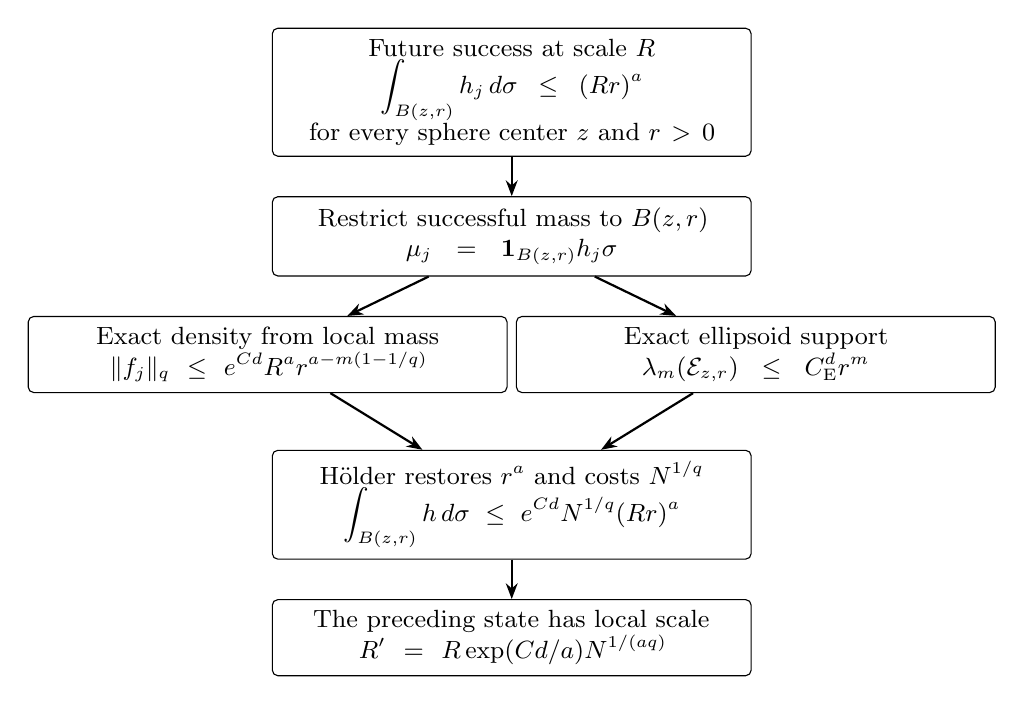
\begin{tikzpicture}[
 box/.style={draw,rounded corners=2pt,align=center,text width=5.8cm,
             inner sep=4pt,font=\small},
 arrow/.style={-{Stealth[length=2mm]},thick},node distance=5mm and 4mm]
\node[box] (local) {Future success at scale \(R\)\\
 \(\displaystyle\int_{B(z,r)}h_j\,d\sigma\le(Rr)^a\)\\
 for every sphere center \(z\) and \(r>0\)};
\node[box,below=of local] (measure) {Restrict successful mass to \(B(z,r)\)\\
 \(\mu_j=\mathbf1_{B(z,r)}h_j\sigma\)};
\node[box,below=of measure,xshift=-3.1cm] (moment) {Exact density from local mass\\
 \(\|f_j\|_q\le e^{Cd}R^a r^{a-m(1-1/q)}\)};
\node[box,below=of measure,xshift=3.1cm] (support) {Exact ellipsoid support\\
 \(\lambda_m(\mathcal E_{z,r})\le C_{\mathrm E}^d r^m\)};
\node[box,below=22mm of measure] (holder) {H\"older restores \(r^a\) and costs \(N^{1/q}\)\\
 \(\displaystyle\int_{B(z,r)}h\,d\sigma\le e^{Cd}N^{1/q}(Rr)^a\)};
\node[box,below=of holder] (output) {The preceding state has local scale\\
 \(R'=R\exp(Cd/a)N^{1/(aq)}\)};
\draw[arrow] (local)--(measure);
\draw[arrow] (measure)--(moment);
\draw[arrow] (measure)--(support);
\draw[arrow] (moment)--(holder);
\draw[arrow] (support)--(holder);
\draw[arrow] (holder)--(output);
\end{tikzpicture}
\caption{The backward block estimate separates the exact projection
density from its common support volume. H\"older combines their radius
powers to recover \(r^a\), while the routing constraint charges
\(N^{1/q}\) for the number of destinations. Absolute constants
\(C\) may change between bounds.}
\label{h:fig:block-scaling}
\end{figure}


In particular, if \(\log N\le d^2\), then
\eqref{h:block:scale} gives \(R'\le KR\) for an absolute \(K\):
the bounds \(a\ge d/3\) and \(q\ge d/16\) make both terms in
\(Cd/a+(\log N)/(aq)\) absolute. This form applies to the local
alphabet whenever \(\log((q+2)2^M)\le d^2\).

For the local count \(N\le(m+2)2^M\) that will be proved in the next
section, \eqref{h:block:scale} gives
\[
 \log(R'/R)
 \le\frac{Cd}{a}+
 \frac{M\log2+\log(m+2)}{aq}
 \le C\left(1+\frac{M}{d^2}\right).
\]
This is where quadratic memory enters: \(q\asymp d\) divides the
logarithm of the number of choices, and \(a\asymp d\) converts mass
growth into scale growth.

\section{From one block to a finite stream}\label{h:stream:section}

The block estimate applies to the success function obtained by starting
the learner from a specified state. We first construct these fresh
continuations and show that a block has only a bounded number of possible
destinations. This count will let us propagate the local bound
\eqref{h:local:bound} backward through the stream.

For now fix the shared rule seed and suppose that all finite transition
and stopping kernels are Borel and defined at every input pair. Future
rows and fresh random choices are independent of the past. We take the
action at the horizon to be terminal from every state.
Section~\ref{h:stream:reduction} justifies these conventions for the full randomized,
completed-measurable model of Definition~\ref{h:model}, without changing
its prior expected terminal score.

\subsection{Fresh continuations and local destinations}

Write $Q_t$ for the set of persistent states at sample index $t$, with
$|Q_t|\le2^M$. For each terminal state $w\in Q_k$, write
$\mathsf Q_{k,w}$ for its output probability law on $S^{d-1}$;
with the seed fixed, this law depends only on $k,w$.
Fix a Borel terminal score
$\ell:S^{d-1}\times S^{d-1}\to[0,1]$. Starting from a specified
state $u\in Q_t$ before its sample-free stopping check, define
$h_{t,u}(s)$ to be the expected terminal score
$\mathbb E[\ell(s,\widehat s)]$ with signal $s$ and fresh future
samples and randomness. This definition also applies to states the
original run never reaches.

A block from index $t$ to index $t+m$ includes the stopping check at
its entrance. An active exit is cut before the check at $t+m$, which
the continuation performs. A terminal tag produced by the last
transition has already stopped at $t+m$. These phase conventions use
only the state and the index.

\begin{lemma}[The destinations of a block]\label{h:stream:categories}
For a fixed-seed Borel learner with the state sets, output laws, and
phase convention just specified, and the Borel terminal score $\ell$, let
$0\le t<T$, $u\in Q_t$, and $1\le m\le T-t$. There are an integer
\begin{equation}\label{h:stream:destinations}
 1\le N\le(m+2)2^M,
\end{equation}
Borel routing functions
$g_j:\mathbb R^{m\times d}\times\mathbb R^m\to[0,1]$ with
$\sum_jg_j\le1$, and Borel functions
$h_j:S^{d-1}\to[0,1]$ such that, for every $s\in S^{d-1}$,
\begin{equation}\label{h:stream:category-representation}
 h_{t,u}(s)=\sum_{j=1}^N h_j(s)
       \int g_j(A,As)\,d\gamma_m(A).
\end{equation}
Here $\gamma_m$ is the law of an $m$-by-$d$ standard Gaussian matrix.
Each destination is either a terminal state $w\in Q_k$ at an index
$k\in\{t,\ldots,t+m\}$, with score function
\[
 h^{\mathrm{out}}_{k,w}(s)
 =\int_{S^{d-1}}\ell(s,v)\,\mathsf Q_{k,w}(dv),
\]
or a continuing state $w\in Q_{t+m}$ before its stopping check, with
score function $h_{t+m,w}(s)$. The terminal output law
$\mathsf Q_{k,w}$ depends only on its state and index. The value
$g_j(A,b)$ is the probability of destination $j$ when the block data
are $(A,b)$.
\end{lemma}

\begin{proof}
The everywhere-defined kernels and the forced terminal action at $T$
give a finite scored experiment from every specified state. Its score
function is Borel in the signal. Indeed, the map
$(s,x)\mapsto(x,\langle x,s\rangle)$ is continuous, and each path
probability is a finite product of Borel coordinate probabilities.
Summing over the finitely many paths and integrating against the fixed
laws of future rows preserves Borel measurability. The same argument
applied to $\ell(s,v)$ and each fixed output law shows that
$h^{\mathrm{out}}_{k,w}$ is Borel. The integration fact follows first
for indicators of rectangles and then for nonnegative Borel functions
by the monotone class theorem and monotone convergence; see also the
composition of kernels in \cite[Section~2.3]{GagnePanangaden2023}.

Pre-generate all $m$ rows of the block, including those after an early
stop. At each $k=t,\ldots,t+m-1$, perform the sample-free stopping
check and, if still active, process the next pair through the transition
to $k+1$. A terminal tag from that transition stops at $k+1$.
An active exit from the final transition is passed to the continuation
before the stopping check at $t+m$, so that check is performed exactly
once. If $t+m=T$, the continuation performs the forced terminal action.

A terminal destination records its local stopping offset
$i\in\{0,\ldots,m\}$ and its terminal state in $Q_{t+i}$.
The offset $i=0$ includes an immediate stop, and $i=m$ can arise
from the last transition. A transition tag and a sample-free stop at
the same state and index have the same output law, so their outcomes
can be merged. Continuing destinations form one additional copy of
$Q_{t+m}$, distinguished from the terminal destinations at that index.
Consequently the number of destinations is at most
\[
 \sum_{i=0}^m|Q_{t+i}|+|Q_{t+m}|\le(m+2)2^M.
\]
The block's entrance index is fixed, so local offsets determine all
absolute stopping indices; the count has no factor depending on $T$.

For arbitrary data $(A,b)$, each destination probability $g_j(A,b)$
is a finite sum over paths of products of Borel coordinate
probabilities. It is therefore Borel. The probabilities are
nonnegative and sum to one when all destinations are included.
A path that stops early is simply independent of the unused rows.
After a continuing destination is fixed, independent future rows and
fresh choices give its prescribed continuation score. After a terminal
destination is fixed, the prescribed output law gives its terminal
score. Conditioning first on the block data and then on its destination
proves \eqref{h:stream:category-representation}. Because the kernels
are defined everywhere, this equality holds for every signal and every
starting state, rather than only at states reached by the original run.
\end{proof}

The angular and chordal success scores are, respectively,
\[
 \ell(s,v)=\mathbf 1_{\{\arccos\langle s,v\rangle\le\epsilon\}},
 \qquad
 \ell(s,v)=\mathbf 1_{\{\|s-v\|\le\epsilon\}}.
\]
Both are Borel. The backward induction below uses the angular score.

\subsection{Borel versions and the original randomized experiment}
\label{h:stream:reduction}

The fresh continuations require kernels defined even at inputs and
states absent from the original run. The model permits transition
coordinates measurable in a completed sigma field. Under a dominated
fresh-pair law, these coordinates admit everywhere-defined Borel
versions that preserve the prior experiment. The following statement
keeps the prior general for the later cube application.


\begin{lemma}[Borel versions under a dominated sample law]
\label{h:stream:borel}
Let $d\ge2$, let $\pi$ be a Borel probability measure on $S^{d-1}$,
and let $X\sim\gamma_1=N(0,I_d)$ be independent of $S\sim\pi$.
Suppose that
\begin{equation}\label{h:stream:pair-domination}
 \mathcal L(X,\langle X,S\rangle)\ll
 \lambda,\qquad \lambda(dx,dy)=\gamma_1(dx)\,dy
\end{equation}
on $\mathbb R^d\times\mathbb R$.
Fix an integer horizon $T\ge0$ and finite state sets at every sample
index. For each state and index, suppose every coordinate of the
finite vector of transition and stopping probabilities is measurable
in the $\lambda$-completion of the Borel sigma field. A terminal output
law is a Borel probability measure on $S^{d-1}$ indexed only by its
terminal state and stopping index. Decisions made without a new sample
also depend only on the state and index.

There are everywhere-defined Borel transition and stopping kernels,
with the same state sets and terminal output laws, whose $\pi$-prior
joint law of the signal, state path, stopping index and output is the
same as for the original rules. The domination
\eqref{h:stream:pair-domination} holds when $\pi=\sigma$ is uniform
spherical probability, for every $d\ge2$.
\end{lemma}

\begin{proof}
We first construct versions for a fixed set of rules. If
$f:\mathbb R^d\times\mathbb R\to[0,1]$ is measurable in the
$\lambda$-completion, each dyadic superlevel set
$\{f\ge k2^{-n}\}$, $1\le k\le2^n$, agrees with a Borel set outside
a Borel $\lambda$-null set, by the description of completion in
Tao~\cite[Exercise~1.4.26]{TaoMeasure2011}. Replace these superlevel sets by their
Borel representatives in
\[
 f_n=2^{-n}\sum_{k=1}^{2^n}\mathbf 1_{\{f\ge k2^{-n}\}}.
\]
The resulting Borel functions have a Borel $\limsup$ equal to $f$
outside the union of the countably many null sets, since $f_n\to f$.
Thus each coordinate of each finite kernel has a Borel version.
For one state and index, choose all of its coordinate versions
simultaneously. The Borel set on which the resulting vector is not
nonnegative with sum one is null; on this set replace the vector by a
fixed point mass. The result is a Borel probability vector at every
sample pair. There are finitely many coordinates, states and indices,
so one Borel $\lambda$-null set $Z$ contains every pair where any
coordinate was changed. Sample-free decisions and terminal output
laws require no such modification.

Pre-generate all $T$ input rows, including rows after an early stop.
Every pair $(X_t,\langle X_t,S\rangle)$ has the marginal law in
\eqref{h:stream:pair-domination}, so
\[
 \mathbb P\{(X_t,\langle X_t,S\rangle)\in Z\}=0.
\]
For a state $u$ chosen from earlier observations, the event that the
learner is in $u$ before sample $t$ and this pair lies in $Z$ is a
subset of the displayed null event. We do not need a density for a
sample conditioned on a particular state. A finite union over $t$
shows that no changed pair is visited almost surely. Couple the
original and modified finite choices by the same uniform random
numbers. Starting from the same initial state, induction makes their
states and stopping decisions equal almost surely. At an equal
terminal state and index the output laws are identical, so use their
diagonal coupling. This proves the asserted joint-law equality. When
$T=0$ there is no sample pair to modify and the same conclusion is
immediate.

It remains to check the spherical prior. Conditional on a nonzero
$X=x$, rotate coordinates so that $x/\|x\|$ is the first coordinate
vector. Write a uniform sphere point as $G/\|G\|$ for a standard
Gaussian vector $G=(G_1,G_\perp)$. When $d\ge2$,
$R=\|G_\perp\|>0$ almost surely and is independent of $G_1$.
For each fixed $R>0$, the map
\[
 g\longmapsto \frac{g}{\sqrt{g^2+R^2}}
\]
is a smooth strictly increasing bijection from $\mathbb R$ to
$(-1,1)$ with nonzero derivative. The image of the Gaussian law of
$G_1$ therefore has a Lebesgue density. Mixing over $R$ and then
multiplying by $\|x\|$ shows that $\langle x,S\rangle$ is absolutely
continuous for every $x\ne0$. The point $x=0$ has $\gamma_1$-measure
zero. Fubini's theorem applied to the sections of a
$\lambda$-null Borel set now proves
\eqref{h:stream:pair-domination}.
\end{proof}

The equality in Lemma~\ref{h:stream:borel} concerns the experiment under
the chosen prior. It need not preserve behavior at every exceptional
individual signal. In particular, an every-signal success premise will
be averaged over the prior before versions are chosen.

We now return to the model's original jointly measurable randomized
experiment. Fix any Borel prior $\pi$ satisfying
\eqref{h:stream:pair-domination}, and draw the signal from $\pi$
independently of the rows and the model's data-independent randomness.
The preceding lemma supplies the domination condition for the
uniform-sphere prior. Write $W$ for the shared rule seed, taking $W$ constant
when no seed is used, and $I$ for its initial state. The observable
signal, rows, state path, stopping index, and output take values in
standard Borel spaces. For a Borel terminal score $\ell$, its original
conditional expectation is a measurable function of $W$ and integrates
to the mixed expected score. Since $(I,W)$ is jointly independent of the signal and all
pre-generated rows, conditional on almost every $W=w$ those inputs
retain their joint law and $I$ is independent of them. The dependence
allowed between $I$ and $W$ does not affect this conclusion.

Fix such a seed value for which the model's per-seed kernel hypotheses
also hold. Lemma~\ref{h:stream:borel}
replaces its completed transition and stopping coordinates by
everywhere-defined Borel kernels while preserving the original
conditional $\pi$-prior law. Keep its terminal output laws. At index $T$,
force the sample-free action to stop at every state, retaining each
prescribed state/index output law. Assign a fixed unit output only where
no law was specified, a case absent from original terminating paths.
This does not change the original conditional
experiment, which already stops by $T$. It makes the horizon convention
in the continuation construction valid even at states absent from that
experiment.

The preceding continuation lemma now applies to this fixed-seed Borel
learner with any Borel terminal score $\ell$. A numerical score bound
uniform over its initial states can be averaged against the conditional
law of $I$. If the bound is also uniform in the fixed seed, the final
seed average uses the original conditional expected scores. Borel
versions may be chosen separately for each seed; no jointly measurable
choice of these replacements is required.

\subsection{The quantitative success bound}

We apply the block bound to the fresh continuations just constructed.
At every step, all terminal destinations have the original terminal
local bound, and all continuing destinations have the inductive bound
at that boundary. The following statement records the resulting
finite-horizon estimate before we extract the sample lower bound.

\begin{proposition}[Success after a bounded number of samples]
\label{h:stream:success}
There are absolute constants $C,d_0>0$ with the following property.
For $d\ge d_0$, every learner in the stated finite-state model with
$M\ge0$ bits and an integer deterministic horizon $T\ge0$ has, for
$S\sim\sigma$ independent of its fresh Gaussian rows,
\begin{equation}\label{h:stream:success-bound}
 \mathbb P\{\arccos\langle\widehat s,S\rangle\le\epsilon\}
 \le
 \min\left\{1,
 \left[2\epsilon\exp\!\left(
 C\left(1+\frac{M}{d^2}\right)
 \left\lceil\frac{T}{q}\right\rceil\right)\right]^a
 \right\},
\end{equation}
where $0<\epsilon\le1/10$ and
$a=(d-1)/2$, $q=\lfloor(d-1)/8\rfloor$ as in
\eqref{h:local:parameters}. The probability includes data-independent
initialization, the shared seed, and fresh random choices.
\end{proposition}

\begin{proof}
Use the angular score in Lemma~\ref{h:stream:categories}. Fix a seed
and a prior-preserving Borel replacement as in
Section~\ref{h:stream:reduction}, with prior $\sigma$.
If $T=0$, its output is a signal-independent mixture of terminal laws.
Lemma~\ref{h:local:caps} gives local mass at scale $\epsilon$.
The radius-two ball about a sphere point covers $S^{d-1}$, so total
success is at most $(2\epsilon)^a$, as required when
$\lceil T/q\rceil=0$. We may now suppose $T\ge1$.

Increase the absolute threshold $d_0$ so that
$q\ge2$, $q\ge d/16$, and $a\ge d/3$. Partition the $T$ sample
indices into $B=\lceil T/q\rceil$ consecutive nonempty blocks, each
of length at most $q$. At the final boundary every continuation is
a terminal output function and obeys \eqref{h:local:bound} at scale
$\epsilon$. Suppose that at the end of one block, all continuing
functions obey that bound at a common scale $R\ge\epsilon$. Its
terminal destinations also obey the bound at scale $R$, by
Lemma~\ref{h:local:caps} and monotonicity in the scale.

For a block of length $m\le q$, Lemma~\ref{h:stream:categories}
places every preceding continuation in the form required by
Lemma~\ref{h:block:bound}, with
$N\le(m+2)2^M\le(q+2)2^M$. That block lemma multiplies the scale
by at most
\[
 \exp(C_0d/a)N^{1/(aq)}
\]
for an absolute $C_0$. Its logarithm is at most
\begin{equation}\label{h:stream:multiplier}
 \frac{C_0d}{a}+
 \frac{M\log2+\log(q+2)}{aq}
 \le C\left(1+\frac{M}{d^2}\right)=:\Lambda,
\end{equation}
where $d/a\le3$, $1/(aq)\le48/d^2$, and
$\log(q+2)/(aq)\le48\log(d+2)/d^2$ allow an absolute $C$.
Backward induction gives \eqref{h:local:bound} at scale
$R=\epsilon e^{\Lambda B}$ for every initial state. Averaging over
the conditional initial-state law preserves this bound, because that
law is independent of the signal and rows. Taking the radius-two ball
gives total success at most $(2\epsilon e^{\Lambda B})^a$, and a
probability is also at most one.

By the reduction in Section~\ref{h:stream:reduction}, this is a
uniform bound on the original conditional success probabilities for
almost every seed. Averaging them proves
\eqref{h:stream:success-bound}; no joint choice of the Borel
replacements is used.
\end{proof}

\section{Constant accuracy and the main lower bound}\label{h:end:section}

Rounding the horizon up to a whole number of blocks loses less than one
block. At fine accuracy this loss is negligible. For the remaining
accuracies, even an estimator retaining all the data needs a linear
number of equations. Reflection across their row span proves this
without identifying the full conditional law of the signal.

\begin{lemma}[Reflection with full data]
\label{h:ev:reflection}
Let \(d\ge1\) be an integer and \(T\ge0\). Let \(S\) be uniform on
\(S^{d-1}\). Let a matrix \(A\) with \(d\) columns, independent of
\(S\), have row span \(U\) of dimension at most \(T\). Suppose an
output \(\widehat S\) is drawn from a probability kernel depending
only on \((A,AS)\). Put \(u=P_US\) and \(v=(I-P_U)S\).
For an arbitrary output in \(\mathbb R^d\) and \(0<\epsilon<1\),
\begin{equation}\label{h:ev:direct-residual}
 \Pr\{\|\widehat S-S\|\le\epsilon\}
 \le\frac12+\frac{T}{2d(1-\epsilon^2)}.
\end{equation}
More generally, for \(0<b_0<1\) and
\(0\le\epsilon<\sqrt{1-b_0}\),
\begin{equation}\label{h:ev:antipodal}
 \Pr\{\|\widehat S-S\|\le\epsilon\}
 \le\frac12+\frac12\Pr\{\|u\|^2\ge b_0\}
 \le\frac12+\frac{T}{2b_0d}.
\end{equation}
For a unit output one also has
\begin{equation}\label{h:ev:reflection-expectation}
 \mathbb E\langle\widehat S,v\rangle=0,\qquad
 \mathbb E\langle\widehat S,S\rangle
 \le\mathbb E\|u\|\le\sqrt{T/d}.
\end{equation}
\end{lemma}

\begin{proof}
The projection \(P_U\) is a Borel function of \(A\), since
\(P_U=\lim_{\eta\downarrow0}A^{\mathsf T}(AA^{\mathsf T}+\eta I)^{-1}A\);
for a matrix with no rows it is zero.
Conditional on \(A\), reflection across \(U\) sends \(S=u+v\) to
\(u-v\). It preserves uniform spherical measure and the data \((A,AS)\),
because \(Av=0\), so the output kernel is the same at both signals.
If \(\|v\|>\epsilon\), the reflected signals have distance greater
than \(2\epsilon\); a fixed estimate can succeed for at most one of
them. Averaging the common output kernel over the reflected pair gives
success at most one half on this event. On its complement use the
bound one. Therefore
\[
 \Pr\{\|\widehat S-S\|\le\epsilon\}
 \le\frac12+\frac12\Pr\{\|u\|^2\ge1-\epsilon^2\}.
\]
Spherical isotropy and independence of \(A\) give
\[
 \mathbb E(\|u\|^2\mid A)=\frac{\dim U}{d}\le\frac Td.
\]
Markov's inequality proves \eqref{h:ev:direct-residual}. The same
pairing on the event \(\|u\|^2<b_0\), where
\(\|v\|>\sqrt{1-b_0}>\epsilon\), proves
\eqref{h:ev:antipodal}. For unit outputs, reflection cancels
\(\mathbb E\langle\widehat S,v\rangle\), whereas
\(\langle\widehat S,u\rangle\le\|u\|\). Cauchy--Schwarz and the
same second-moment identity prove \eqref{h:ev:reflection-expectation}.
\end{proof}

For almost every fixed shared seed, use the prior-preserving Borel
rules justified in Section~\ref{h:stream:section}. Pre-generate all
\(T\) Gaussian rows and grant the learner the full matrix and labels.
After averaging its signal-independent initial state and fresh choices,
its stopped output law is a Borel kernel of those data. Angular error
at most \(\epsilon\) implies Euclidean error at most \(\epsilon\).
If \(T\le d/4\) and \(\epsilon\le1/10\), then
\eqref{h:ev:direct-residual} gives success probability at most
\[
 \frac12+\frac1{8(1-\epsilon^2)}
 \le\frac{62}{99}<\frac23.
\]
This uniform bound also holds for the original conditional success
probabilities and hence for their average over the seed. Thus any
learner with the stipulated average success must satisfy
\begin{equation}\label{h:end:linear-threshold}
 T>d/4.
\end{equation}

\begin{proof}[Proof of Theorem~\ref{h:main}]
Fix the finite constant \(A>0\) in the theorem. Take \(d\) above
the absolute threshold in Proposition~\ref{h:stream:success}, and
large enough that \(a\ge1\) and \(q\ge d/16\). Put
\[
 K_A=\exp(C(1+A))>1,\qquad
 L=\log(1/\epsilon),\qquad B=\lceil T/q\rceil,
\]
where \(C\) is the absolute constant in that proposition. Since
\(M\le Ad^2\) and prior success is at least \(2/3\),
\[
 \frac23\le(2\epsilon K_A^B)^a.
\]
Taking the \(a\)th root gives \(\epsilon K_A^B\ge1/3\).
Since \(B\le T/q+1\),
\begin{equation}\label{h:end:rounding}
 T\ge q\left(\frac{L-\log3}{\log K_A}-1\right).
\end{equation}
Let \(H_A=2(\log3+\log K_A)\). If \(L\ge H_A\), this gives
\[
 T\ge\frac{qL}{2\log K_A}\ge\frac{dL}{32\log K_A}.
\]
If \(L<H_A\), \eqref{h:end:linear-threshold} instead gives
\(T>d/4>dL/(4H_A)\). Thus the same choice
\[
 c_A=\min\left\{\frac1{32\log K_A},\frac1{4H_A}\right\}>0
\]
works uniformly over \(0<\epsilon\le1/10\) and \(M\le Ad^2\)
for this fixed \(A\). No positive constant uniform as \(A\) tends
to infinity is asserted.
\end{proof}

\begin{proof}[Proof of Corollary~\ref{h:subquadratic}]
Since $M(d)=o(d^2)$, there is a dimension $d_M$ after which
$M(d)\le d^2$. Apply Theorem~\ref{h:main} with the numerical choice
$A=1$ at every $d\ge d_M$, so $K_1=e^{2C}$ in the preceding proof.
Its constant $c_1$ is absolute, and the
eventual dimension threshold may depend on the memory sequence
through $d_M$. The argument applies separately at every accuracy
$0<\epsilon(d)\le1/10$, so it requires neither monotonicity of that
sequence nor a relation between memory and accuracy.
\end{proof}

\begin{proof}[Proof of Corollary~\ref{h:worst-signal}]
Average the original fixed-signal experiment over $S\sim\sigma$
before choosing Borel versions. Its measurability makes the resulting
success probability the integral of the fixed-signal success
probabilities. A success probability at least $2/3$ for every
signal therefore gives uniform-prior success at least $2/3$.
Theorem~\ref{h:main} and Corollary~\ref{h:subquadratic} give the
corresponding conclusions with their unchanged constants and
dimension thresholds. Lemma~\ref{h:stream:borel} preserves the
average used in those arguments even if a version changes behavior
at exceptional individual signals.
\end{proof}

\section{Selection on a common data domain}
\label{h:alternatives}

The two applications use the same analytic selection step: several
continuation measures are supported on one data domain, and a measurable
route chooses among them. The strong density estimate of
Theorem~\ref{h:dv:finite-density} is sufficient, but a bound for
measurable tests already gives the required \(N^{1/p}\) cost.

We state this common step before applying the projection theorem to a
lower-dimensional cube prior in Section~\ref{h:cube:section}.
The later sections examine additional exact-label interfaces and
alternative coefficient normalizations; they do not assert a stronger
main theorem.

\begin{lemma}[Selection on a common data domain]\label{h:alt:selection}
Let \((E,\mathcal E,\lambda)\) be a measure space, let
\(\mathcal D\in\mathcal E\) have finite measure, let \(p>1\), let
\(U\ge0\), and let \(N\ge1\) be an integer. Suppose finite nonnegative measures
\(\eta_1,\ldots,\eta_N\) are supported on \(\mathcal D\), and that
for every measurable \(0\le g\le1\),
\begin{equation}\label{h:alt:test}
 \int g\,d\eta_j
 \le U\left(\int_{\mathcal D}g\,d\lambda\right)^{1-1/p}
 \qquad(1\le j\le N).
\end{equation}
For measurable routes \(g_j\ge0\) with \(\sum_jg_j\le1\),
\begin{equation}\label{h:alt:selection-bound}
 \sum_{j=1}^N\int g_j\,d\eta_j
 \le N^{1/p}U\,\lambda(\mathcal D)^{1-1/p}.
\end{equation}
A sufficient condition for \eqref{h:alt:test} is
\(\eta_j=f_j\lambda\), where \(f_j\ge0\) vanishes outside
\(\mathcal D\) and \(\|f_j\|_{L^p(\lambda)}\le U\).

In particular, if \(r>0\), \(m,\beta\in\R\), and positive constants
\(H,V,L\) satisfy
\[
 U\le HLr^{\beta-m(1-1/p)},\qquad
 \lambda(\mathcal D)\le Vr^m,
\]
then the right side of \eqref{h:alt:selection-bound} is at most
\begin{equation}\label{h:alt:scale-cancellation}
 N^{1/p}H V^{1-1/p}Lr^\beta.
\end{equation}
\end{lemma}

\begin{proof}
Each \(g_j\) lies in \([0,1]\). Put
\(b_j=\int_{\mathcal D}g_j\,d\lambda\). Equation
\eqref{h:alt:test} and H\"older on the finite index set give
\[
 \sum_j\int g_j\,d\eta_j
 \le U\sum_jb_j^{1-1/p}
 \le U N^{1/p}\left(\sum_jb_j\right)^{1-1/p}.
\]
Since \(\sum_jg_j\le1\), we have
\(\sum_jb_j\le\lambda(\mathcal D)\), proving
\eqref{h:alt:selection-bound}. Under the density condition,
H\"older gives
\[
 \int g\,d\eta_j
 \le U\left(\int_{\mathcal D}g^{p/(p-1)}\,d\lambda\right)^{1-1/p}
 \le U\left(\int_{\mathcal D}g\,d\lambda\right)^{1-1/p},
\]
because \(0\le g\le1\). Finally the powers of \(r\) in the two
assumed bounds add to \(\beta\), giving
\eqref{h:alt:scale-cancellation}.
\end{proof}

The test formulation accommodates a direct open-set limit even when
one chooses not to infer a strong \(L^p\) density from that limit.
The density formulation applies to the other passages. In both cases,
the reference measure and the common support must be the ones
specified by the corresponding projection estimate.

\section{A paired-coordinate cube application}\label{h:cube:section}

The exact-density theorem for finite measures also applies to a prior
supported on a lower-dimensional subset of the sphere.  We illustrate
this with a cube embedded by coordinate pairs.  Its first coordinates
transfer the local mass bound to ambient Euclidean balls, and its
Lipschitz bound supplies a common support for the projected labels.
These are the hypotheses needed by the general projection and selection
estimates.

The resulting success bound concerns the cube prior.  It gives a
sample lower bound at fine accuracy from cube-average success alone.
To cover the remaining accuracies for a learner that succeeds at every
unit signal, we use the uniform-sphere endpoint from the main proof.

\subsection{The prior and its terminal mass}

Let \(d\ge16\) be an integer, set \(n=\lfloor d/2\rfloor\), and give
\[
 Q=[-1/2,1/2]^n
\]
Lebesgue probability measure \(du\).  The cube has volume one.  Define
\begin{equation}\label{h:cube:map}
 \iota(u)=\frac1{\sqrt n}
 \bigl(u_1,\ldots,u_n,\sqrt{1-u_1^2},\ldots,
       \sqrt{1-u_n^2},0,\ldots,0\bigr)\in\mathbb R^d,
\end{equation}
with \(d-2n\) zero coordinates.  Each coordinate pair contributes
\(1/n\) to the squared norm, so \(\iota(Q)\subset S^{d-1}\).
The signal prior is \(\iota_\#du\).

Write \(\operatorname{pr}:\mathbb R^d\to\mathbb R^n\) for projection
onto the first \(n\) coordinates.  Then
\(\operatorname{pr}\iota(u)=u/\sqrt n\).  On \([-1/2,1/2]\), the
derivative of \(a\mapsto\sqrt{1-a^2}\) has absolute value at most
\(1/\sqrt3\).  The mean value theorem therefore gives
\begin{equation}\label{h:cube:lipschitz}
 \|\iota(u)-\iota(v)\|\le\frac2{\sqrt n}\|u-v\|
 \qquad(u,v\in Q).
\end{equation}

Set
\begin{equation}\label{h:cube:parameters}
 \alpha=\frac n4,\qquad \beta=n-\alpha=\frac{3n}{4},
 \qquad p=\left\lfloor\frac n4\right\rfloor\ge2.
\end{equation}
For \(z\in\mathbb R^n\) and \(r>0\), abbreviate
\[
 \mathcal B(z,r)=Q\cap B_n(z,\sqrt n\,r),
\]
where \(B_j(x,t)\) is the closed Euclidean ball in \(\mathbb R^j\).
The local bound for a function \(f:Q\to[0,1]\) will be
\begin{equation}\label{h:cube:local}
 \int_{\mathcal B(z,r)}f(u)\,du\le Lr^\beta
 \qquad(z\in\mathbb R^n,\ r>0).
\end{equation}
We will propagate the coefficient \(L\) backward through the stream.

Fix a terminal state and stopping index, after fixing the independent
rule seed.  Its output law is independent of the signal.  Let
\(f_{\rm term}(u)\) be the probability that this output has angular
error at most \(\epsilon\) at \(\iota(u)\).  For a fixed unit output
\(\widehat s\), angular error at most \(\epsilon\) implies
chordal error at most \(\epsilon\).  Projection onto the first
coordinates then gives
\[
 \|u-\sqrt n\,\operatorname{pr}\widehat s\|
 \le\sqrt n\,\epsilon.
\]
Let \(\omega_j\) be the volume of the unit ball in \(\mathbb R^j\).
The Gaussian integral gives
\(\omega_j j^{j/2}\le(2\pi e)^{j/2}\): integrate
\(e^{-\|x\|^2/2}\) over the ball of radius \(\sqrt j\) and compare
with its integral over \(\mathbb R^j\).  The successful part of
\(\mathcal B(z,r)\) lies in two parameter balls, so its volume is at
most the smaller of their volumes.  With \(C_0=\sqrt{2\pi e}\), the
terminal success function consequently satisfies
\begin{equation}\label{h:cube:terminal}
 \int_{\mathcal B(z,r)}f_{\rm term}(u)\,du
 \le C_0^n\min(r,\epsilon)^n
 \le C_0^n\epsilon^\alpha r^\beta.
\end{equation}
The last inequality uses \(\alpha+\beta=n\); the same estimate for a
random output follows by integration against its signal-independent law.

\subsection{Transferring local mass to the embedded measure}

Let \(\gamma_k\) be the law of a \(k\)-by-\(d\) matrix with
independent standard Gaussian entries, and put
\[
 \lambda_k(dA,dy)=\gamma_k(dA)\,dy.
\]
The following specialization supplies both the exact density and its
common support.  A parameter function measurable in the Lebesgue
completion can first be replaced by a Borel version under \(du\),
without changing any local integral.

\begin{lemma}[Exact density and a common projected ellipsoid]
\label{h:cube:density}
Let \(k\) be an integer with \(1\le k\le p\), and let a Borel function
\(f:Q\to[0,1]\) satisfy \eqref{h:cube:local} with \(L\ge0\).
For \(z\in\mathbb R^n\) and \(r>0\), define the finite joint measure
\begin{equation}\label{h:cube:joint-measure}
 \eta_{f,z,r}(E)
 =\int\!\int_{\mathcal B(z,r)}
       \mathbf 1_E(A,A\iota(u))f(u)\,du\,\gamma_k(dA)
\end{equation}
for Borel \(E\subseteq\mathbb R^{k\times d}\times\mathbb R^k\).
There is a universal \(C_2\ge1\) such that
\(\eta_{f,z,r}=h_{f,z,r}\lambda_k\) for a nonnegative density with
\begin{equation}\label{h:cube:density-bound}
 \|h_{f,z,r}\|_{L^p(\lambda_k)}
 \le C_2^n Lr^{\beta-k(1-1/p)}.
\end{equation}
If \(\mathcal B(z,r)\ne\varnothing\), fix any
\(u_*\in\mathcal B(z,r)\) and set
\begin{equation}\label{h:cube:ellipsoid-support}
 \mathcal E_{u_*,r}
 =\{(A,y):y\in A\iota(u_*)+A B_d(0,4r)\}.
\end{equation}
Every such density, for this same \(z,r,u_*\), vanishes almost
everywhere outside \(\mathcal E_{u_*,r}\), and
\begin{equation}\label{h:cube:ellipsoid-volume}
 \lambda_k(\mathcal E_{u_*,r})\le C_2^n r^k.
\end{equation}
\end{lemma}

\begin{proof}
An empty \(\mathcal B(z,r)\) gives the zero measure.  Otherwise fix
\(u_*\in\mathcal B(z,r)\), and let
\[
 \mu=\iota_\#\bigl(\mathbf1_{\mathcal B(z,r)}f(u)\,du\bigr).
\]
For any \(x\in\mathbb R^d\) and \(t>0\), projection onto the first
coordinates gives
\begin{equation}\label{h:cube:ambient-growth}
 \begin{split}
 \mu(B_d(x,t))
 &\le\int_{\mathcal B(\sqrt n\,\operatorname{pr}x,t)}f(u)\,du\\
 &\le Lt^\beta.
 \end{split}
\end{equation}
For \(u\in\mathcal B(z,r)\), the distance from \(u\) to \(u_*\) is
at most \(2\sqrt n\,r\).  Thus \eqref{h:cube:lipschitz} puts
\(\mu\) inside \(B_d(\iota(u_*),4r)\).

If \(L=0\), \eqref{h:cube:local} applied to a ball containing \(Q\)
gives \(f=0\) almost everywhere, and the zero density suffices.  Suppose
now that \(L>0\).  Apply the general finite-measure result
Theorem~\ref{h:dv:finite-density} with
\[
 H=L,\qquad R=4r,\qquad m=k,
 \qquad \beta=3n/4,\qquad p=\lfloor n/4\rfloor.
\]
For its factors \(J_j\), the required margin and their uniform bounds
are
\begin{equation}\label{h:cube:margin}
 \beta-j-k\ge\frac{3n}{4}-2p+2\ge\frac n4+2,
 \qquad
 J_j=1+3^j2^\beta\frac{k}{\beta-j-k}
 \le1+3^{n/4}2^{3n/4}
 \qquad(0\le j\le p-2).
\end{equation}
In particular \(\beta>k+p-2\).  We use the general parameter range
of that theorem, not the specialization to exponents near half
the ambient dimension.
Its exact norm bound is
\[
 (2\pi)^{-k(p-1)/(2p)}
 L(4r)^{\beta-k(1-1/p)}
 \left(\prod_{j=0}^{p-2}J_j\right)^{1/p}.
\]
The first factor is at most one, each \(J_j\le C^n\), and
\(0<\beta-k(1-1/p)\le\beta\).  Absorbing
\(4^{\beta-k(1-1/p)}\le4^\beta\) into \(C_2^n\) proves
\eqref{h:cube:density-bound}.  This is the density of the exact joint
measure \eqref{h:cube:joint-measure}; no density relative to spherical
area is assumed.

The set \(\mathcal E_{u_*,r}\) is the exact projected image of the
enclosing ball \(B_d(\iota(u_*),4r)\).  Lemma~\ref{h:ev:ellipsoid}
makes this set Borel and gives the asserted common support.  The same
lemma gives
\[
 \lambda_k(\mathcal E_{u_*,r})
 \le C_{\mathrm E}^d(4r)^k\le C_2^n r^k,
\]
after one universal increase of \(C_2\), since
\(d\le2n+1\) and \(k\le n/4\).  This calculation also covers the
zero-density case.
\end{proof}

\subsection{The block bound and the streaming consequence}

The power of \(r\) lost in the density norm is restored by the common
support volume.  Selection then costs only the \(p\)th root of the
number of continuations.

\begin{corollary}[A block on the paired-coordinate prior]
\label{h:cube:block}
Let \(k,N\) be integers with \(1\le k\le p\) and \(N\ge1\), and let Borel
\(f_1,\ldots,f_N:Q\to[0,1]\) satisfy \eqref{h:cube:local} with the
same \(L\ge0\).  Suppose Borel functions
\(g_v:\mathbb R^{k\times d}\times\mathbb R^k\to[0,\infty)\) obey
\(\sum_{v=1}^N g_v(A,y)\le1\).  Then
\[
 F(u)=\mathbb E_{A\sim\gamma_k}
       \sum_{v=1}^N g_v(A,A\iota(u))f_v(u)
\]
satisfies \eqref{h:cube:local} with \(C_3^nN^{1/p}L\) in place of
\(L\), for a universal \(C_3\ge1\).
\end{corollary}

\begin{proof}
Fix \(z,r\).  An empty \(\mathcal B(z,r)\) is immediate.  Otherwise
choose the same \(u_*\in\mathcal B(z,r)\) for all \(v\).  The exact
joint densities from Lemma~\ref{h:cube:density} share its region
\(\mathcal E_{u_*,r}\).  Apply
Lemma~\ref{h:alt:selection} with density norm at most
\(C_2^nLr^{\beta-k(1-1/p)}\) and domain measure at most
\(C_2^nr^k\).  The image-measure identity and that lemma give
\begin{equation}\label{h:cube:selection}
 \int_{\mathcal B(z,r)}F(u)\,du
 \le N^{1/p}C_2^n(C_2^n)^{1-1/p}Lr^\beta
 \le C_3^nN^{1/p}Lr^\beta.
\end{equation}
The radius powers cancel, and the same \(C_3\) works for every
\(1\le k\le p\).
\end{proof}

To apply this bound to the model's completed-measurable rules, first
observe that \(f=1\) satisfies
\[
 |\mathcal B(z,r)|\le\min\{1,C_0^nr^n\}\le C_0^nr^\beta.
\]
Take \(k=1\) in Lemma~\ref{h:cube:density} and a parameter ball
containing \(Q\).  The fresh pair
\((X,\langle X,\iota(u)\rangle)\), for \(u\sim du\), is therefore
absolutely continuous relative to \(\gamma_1(dx)\,dy\).
We may consequently use the seedwise Borel reduction and fresh-state
continuations of Section~\ref{h:stream:reduction} under this cube prior.
As there, the conditional numerical estimates are averaged using the
original measurable experiment; no jointly chosen family of Borel
replacements is required.

\Needspace{4\baselineskip}
\begin{proposition}[Precision bound for the cube prior]
\label{h:cube:success}
There are universal constants \(D\ge e\), \(d_0\ge16\), and \(c>0\)
with the following property.  Let \(d\ge d_0\), \(M\ge0\), and \(T\ge0\)
be integers, with \(M\le d^2\) and \(0<\epsilon\le1/10\).
Every learner in Definition~\ref{h:model} with these memory and sample
bounds has angular success probability under \(s=\iota(u)\), \(u\sim du\),
at most
\begin{equation}\label{h:cube:success-bound}
 \min\left\{1,\,
       D^{n(m+1)}\epsilon^{n/4}\right\},
 \qquad
 m=\left\lceil\frac{T}{k_0}\right\rceil,\qquad
 k_0=\left\lfloor\frac n4\right\rfloor.
\end{equation}
The probability averages over \(u\), the fresh Gaussian samples, and
the learner's randomness.  If that same learner has angular success
probability at least \(2/3\) for every \(s\in S^{d-1}\), then
\begin{equation}\label{h:cube:sample-result}
 T\ge c\,d\log(1/\epsilon).
\end{equation}
\end{proposition}

\begin{proof}
Use the seedwise convention just established, and first start from any
prescribed initial state.  For \(T>0\), partition the stream into
\(m=\lceil T/p\rceil\) consecutive blocks, each of length at most
\(p=k_0\).  Lemma~\ref{h:stream:categories}, with angular terminal
score and signal \(\iota(u)\), represents the preceding success
function by the exact block formula in Corollary~\ref{h:cube:block}.
For a block of length \(k\), its Borel routes have at most
\begin{equation}\label{h:cube:destinations}
 N\le(k+2)2^M
\end{equation}
destinations.  The stopping offsets are local to this block, including
an immediate stop; its continuing functions use fresh future samples.
These are the same phase and terminal-state conventions as in that
lemma.

For \(n\ge8\), \(p\ge n/8\), \(d\le2n+1\), and \(M\le d^2\),
\[
 \frac{\log N}{p}
 \le\frac{d^2\log2+\log(p+2)}p\le C_4n
\]
with a universal \(C_4\).  Choose a universal \(D\ge e\) so that
\(D\ge C_0\) and \(C_3^nN^{1/p}\le D^n\).
The terminal coefficient is \(C_0^n\epsilon^{n/4}\) by
\eqref{h:cube:terminal}.  Backward induction, applying the block bound
and retaining the terminal estimate at earlier stops, gives coefficient
\[
 L=D^{n(m+1)}\epsilon^{n/4}
\]
for every initial state.  The ball \(\mathcal B(0,1)\) contains \(Q\),
so this coefficient bounds total cube-average success.  For \(T=0\),
the terminal bound gives the same statement with \(m=0\).
All constants are uniform over the seedwise Borel rules and prescribed
states.  The independent conditional initialization and the averaging
of original conditional success probabilities from
Section~\ref{h:stream:reduction} therefore prove
\eqref{h:cube:success-bound} for the original learner, including every
short last block.

Suppose now only that the cube-average success is at least \(2/3\).
Taking natural logarithms in \eqref{h:cube:success-bound} and using
\(m\le T/k_0+1\) gives
\begin{equation}\label{h:cube:sample-bound}
 \frac{T}{k_0}
 \ge\frac{\log(1/\epsilon)}{4\log D}
       -2-\frac{\log(3/2)}{n\log D}.
\end{equation}
If \(\log(1/\epsilon)\ge24\log D\), its right side is at least
\(\log(1/\epsilon)/(8\log D)\).  Since \(k_0\ge n/8\) and
\(n\ge d/3\), this already gives
\(T\ge d\log(1/\epsilon)/(192\log D)\) in that accuracy range.

For the all-accuracy conclusion \eqref{h:cube:sample-result}, assume
the stated every-signal guarantee.  It gives the cube-average premise
just used.  It also gives uniform-sphere average success at least
\(2/3\) for the same original learner.  The reflection consequence
\eqref{h:end:linear-threshold} therefore forces \(T>d/4\).
For \(\log(1/\epsilon)<24\log D\), this implies
\[
 T>\frac d4>\frac{d\log(1/\epsilon)}{96\log D}.
\]
Combining the two ranges proves \eqref{h:cube:sample-result}, for
example with \(c=1/(192\log D)\), after increasing the universal
dimension threshold as needed.  The memory condition \(M\le d^2\)
in particular holds eventually for every sequence \(M(d)=o(d^2)\).
\end{proof}

\subsection{An affine-distance interpretation}

The application is complete.  The embedding also gives a direct
interpretation of the Gram moment behind its projection bound.  This
alternative calculation isolates what the first coordinates guarantee
about affine spans.  For \(u,u_1,\ldots,u_j\in Q\), \(j\ge1\),
\begin{equation}\label{h:cube:affine}
 \operatorname{dist}\bigl(\iota(u),
       \operatorname{aff}(\iota(u_1),\ldots,\iota(u_j))\bigr)
 \ge\frac1{\sqrt n}
       \operatorname{dist}\bigl(u,\operatorname{aff}(u_1,\ldots,u_j)\bigr).
\end{equation}
Indeed, for \(\sum_i c_i=1\), projection of
\(\iota(u)-\sum_i c_i\iota(u_i)\) is
\((u-\sum_i c_i u_i)/\sqrt n\).  Projection cannot increase norm,
and taking the infimum proves the claim, including dependent points.

\begin{lemma}[Affine inverse moments]\label{h:cube:inverse}
Let \(f:Q\to[0,1]\) be Borel and satisfy \eqref{h:cube:local} with
\(L\ge0\).  Let \(k\) be an integer with \(1\le k\le p\), and let
\(V\subseteq\mathbb R^n\) be a nonempty affine subspace of dimension
\(j\le p-2\).  There is a universal \(C_1\ge1\) such that, for every
\(z\in\mathbb R^n\), \(r>0\), and \(0<t\le1\),
\begin{align}
 \int_{\mathcal B(z,r)}f(u)
   \mathbf1_{\{\operatorname{dist}(u,V)\le\sqrt n\,tr\}}\,du
 &\le C_1^n Lr^\beta t^{\beta-j},
 \label{h:cube:tube}\\
 \int_{\mathcal B(z,r)}f(u)
   \left(\frac{\operatorname{dist}(u,V)}{\sqrt n}\right)^{-k}\,du
 &\le C_1^n Lr^{\beta-k}.
 \label{h:cube:inverse-bound}
\end{align}
The second integrand is nonnegative and extended-valued on \(V\).
\end{lemma}

\begin{proof}
The cases \(L=0\) and an empty parameter ball are immediate as above.
Apply Proposition~\ref{h:dv:ambient-gram} in parameter dimension
\(n\) to
\(\mathbf1_{\mathcal B(z,r)}f(u)\,du\), with
\[
 H=Ln^{-\beta/2},\qquad R=\sqrt n\,r,\qquad m=k.
\]
The growth hypothesis follows because a parameter ball of radius
\(a>0\) is \(\mathcal B(x,a/\sqrt n)\) after intersection with
\(Q\).  Its tube bound, evaluated at \(\sqrt n\,tr\), is
\[
 3^j2^\beta (Ln^{-\beta/2})(\sqrt n\,r)^j
                 (\sqrt n\,tr)^{\beta-j}
 =3^j2^\beta Lr^\beta t^{\beta-j}.
\]
Its inverse-distance bound is
\(J_jLn^{-k/2}r^{\beta-k}\).  Multiplication by \(n^{k/2}\)
gives the normalization in \eqref{h:cube:inverse-bound}.
The bounds \eqref{h:cube:margin} absorb both constants into a universal
\(C_1^n\).
\end{proof}

For example, let \(G\) be the Gram matrix of the \(p-1\) differences
\(\iota(u_i)-\iota(u_1)\), \(2\le i\le p\).
Almost every parameter tuple is affinely independent, since proper
affine subspaces of \(\mathbb R^n\) have zero Lebesgue measure.
Writing \(V_{i-1}=\operatorname{aff}(u_1,\ldots,u_{i-1})\),
Gram--Schmidt and \eqref{h:cube:affine} give
\begin{equation}\label{h:cube:gram}
 \det G\ge
 \prod_{i=2}^p
 \left(\frac{\operatorname{dist}(u_i,V_{i-1})}{\sqrt n}\right)^2>0.
\end{equation}
Integrating in the order \(u_p,\ldots,u_2\), followed by \(u_1\),
therefore yields
\[
 \int_{\mathcal B(z,r)^p}\det G^{-k/2}
             \prod_{i=1}^p f(u_i)\,du_1\cdots du_p
 \le C_1^{n(p-1)}L^p r^{\beta p-k(p-1)}.
\]
Thus one can also obtain the projection bound by inserting this Gram
estimate into the Gaussian difference identity and compact-test passage
of Section~\ref{h:projection}.  The main application instead uses the
general finite-measure theorem through the ambient ball bound
\eqref{h:cube:ambient-growth}.

\paragraph{An enclosing-ball alternative.}
The common ellipsoid may instead be enclosed in the larger label ball
\begin{equation}\label{h:cube:support}
 \mathcal R_A=B_k\bigl(A\iota(u_*),4r\|A\|_{\rm op}\bigr).
\end{equation}
Thus every density in Lemma~\ref{h:cube:density}, with the same
\(z,r,u_*\), also vanishes almost everywhere outside
\(\{(A,y):y\in\mathcal R_A\}\).  Its volume has the bound
\begin{equation}\label{h:cube:volume}
 \mathbb E_{A\sim\gamma_k}|\mathcal R_A|
 =(4r)^k\mathbb E\,\vol_k B_k(0,\|A\|_{\rm op})
 \le4^k e^{Cd}r^k\le C_2^n r^k,
\end{equation}
after a universal increase of \(C_2\), where
\(|\mathcal R_A|\) is \(k\)-dimensional Lebesgue volume.
This estimate follows independently from the Gaussian net bound in
Lemma~\ref{h:proj:volume}, not from the smaller ellipsoid's volume.
It gives the same block bound, although the direct proof above uses
the exact projected ellipsoid and does not require this enlargement.

\appendix
\section{Other exact-label interfaces}
\label{h:dv:section}

Theorem~\ref{h:dv:finite-density} supplies the strong joint \(L^p\)
density used in both applications. We now separate three additional
conclusions that need not be built into that theorem. A direct
difference-kernel argument proves the measurable-test estimate needed
for selection without using compact-test duality. For spherical
restrictions, joint \(L^1\) convergence identifies the limiting density;
a specified pointwise version works for every full-row-rank matrix,
rather than only almost every matrix.

We retain the notation \(\eta_\mu,\lambda_m,\mathcal E_{z,R}\) of
Section~\ref{h:projection} and the exact norm scale \(\mathcal B\)
in \eqref{h:dv:moment-scale}. The coefficient \(H\) controls mass in
all ambient balls, while \(R\) is the radius of a supporting ball;
neither measure is normalized to a posterior.

\subsection{A direct bound for measurable tests}

\begin{proposition}[A direct inequality for measurable tests]
\label{h:dv:measurable-test}
Under the assumptions of Proposition~\ref{h:dv:ambient-gram}, the
exact image measure satisfies
\begin{equation}
 \eta_\mu(E)\le \mathcal B\,\lambda_m(E)^{1-1/p}
 \label{h:dv:set-bound}
\end{equation}
for every Borel set \(E\) of finite \(\lambda_m\)-measure.  In
particular \(\eta_\mu\ll\lambda_m\), and the same inequality holds on
the \(\lambda_m\)-completion after extending \(\eta_\mu\) to that
completion.  For every \(\lambda_m\)-completed-measurable
\(0\le\varphi\le1\),
\begin{equation}
 \int\varphi\,d\eta_\mu
 \le\mathcal B
 \left(\int_{\mathcal E_{z,R}}\varphi\,d\lambda_m\right)^{1-1/p}.
 \label{h:dv:test-bound}
\end{equation}
An infinite integral on the right is allowed.
\end{proposition}

\begin{proof}
Let \(\rho_\delta=(v_m\delta^m)^{-1}
\mathbf1_{B(0,\delta)}\) be the uniform probability density of the
radius-\(\delta\) ball in \(\mathbb R^m\), and set
\(U_\delta(A,y)=\int\rho_\delta(y-As)\,d\mu(s)\).
After translating the common label variable by \(As_1\), the tuple
kernel in its \(p\)th moment becomes
\[
 K_\delta(v_2,\ldots,v_p)
 =\int_{\mathbb R^m}\rho_\delta(b)
       \prod_{i=2}^p\rho_\delta(b-v_i)\,db,
 \qquad v_i=A(s_i-s_1).
\]
It is nonnegative, and Tonelli's theorem gives the exact normalization
\begin{equation}
 \int_{\mathbb R^{m(p-1)}}K_\delta(v_2,\ldots,v_p)
       \,dv_2\cdots dv_p=1.
 \label{h:dv:difference-kernel}
\end{equation}
In particular the kernel depends on \(A\) only through the differences;
no independence of \(As_1\) from those differences is used.

For a full-rank \(V\), the rows of \(AV\) are independent centered
Gaussian vectors with covariance \(V^{\mathsf T}V\).  Their joint
density has supremum
\((2\pi)^{-m(p-1)/2}\det(V^{\mathsf T}V)^{-m/2}\).
Multiplying this density by the unit-mass kernel
\eqref{h:dv:difference-kernel} bounds the expected tuple kernel by
that supremum.  Expand \(\int U_\delta^p\,d\lambda_m\), discard only
the product-null rank exceptions, and apply
\eqref{h:dv:gram-product}.  This gives
\begin{equation}
 \|U_\delta\|_{L^p(\lambda_m)}\le\mathcal B
 \qquad(\delta>0).
 \label{h:dv:difference-moment}
\end{equation}

The measure \(\lambda_m\) is Borel and finite on compact sets in a
Euclidean space.  The Radon extension theorem
\cite[Corollary~2.11]{StanfordRadonMeasures} applies and gives outer
regularity on Borel sets.  If \(O\) is open, then for
each \((A,As)\in O\), all sufficiently small label perturbations
remain in \(O\).  Fatou's lemma followed by H\"older's inequality gives
\[
 \eta_\mu(O)
 \le\liminf_{\delta\downarrow0}\int_O U_\delta\,d\lambda_m
 \le\mathcal B\,\lambda_m(O)^{1-1/p}.
\]
For a Borel \(E\) with finite \(\lambda_m(E)\), take open supersets
whose \(\lambda_m\)-measures decrease to \(\lambda_m(E)\).  The last
inequality proves \eqref{h:dv:set-bound}.  Applied to null sets, it
gives \(\eta_\mu\ll\lambda_m\).  Extending \(\eta_\mu\) by zero on
\(\lambda_m\)-null sets gives the asserted version on the
\(\lambda_m\)-completion.

The measure \(\eta_\mu\) is supported on the Borel set
\(\mathcal E_{z,R}\).  If
\(\int_{\mathcal E_{z,R}}\varphi\,d\lambda_m<\infty\), apply
\eqref{h:dv:set-bound} to
\(\{\varphi>t\}\cap\mathcal E_{z,R}\) for \(t>0\).  Layer cake and
concavity of \(x^{1-1/p}\) yield
\begin{align*}
 \int\varphi\,d\eta_\mu
 &\le\mathcal B\int_0^1
   \lambda_m(\{\varphi>t\}\cap\mathcal E_{z,R})^{1-1/p}\,dt\\
 &\le\mathcal B
   \left(\int_0^1
   \lambda_m(\{\varphi>t\}\cap\mathcal E_{z,R})\,dt\right)^{1-1/p},
\end{align*}
which is \eqref{h:dv:test-bound}.  The case of an infinite right side
is immediate.  This proof supplies the measurable-test estimate
directly; it does not infer a strong \(L^p\) bound from the set
inequality alone.
\end{proof}

\subsection{Spherical absolute continuity and compatible fibers}

The remaining constructions use an additional hypothesis:
\(\mu\ll\sigma_d\) and \(m<d\). It provides absolute continuity for
each full-row-rank matrix separately. This hypothesis is not needed
by the general finite-measure theorem or the preceding direct-test
bound.

\begin{lemma}[Absolute continuity of spherical projections]
\label{h:dv:gaussian-ac}
Let \(d\ge2\) and \(1\le m<d\).  If \(A:\mathbb R^d\to\mathbb R^m\)
has full row rank, then \(A_\#\sigma_d\) is absolutely continuous with
respect to Lebesgue measure.  The same holds for \(A_\#\mu\) whenever
\(\mu\) is a finite Borel measure with \(\mu\ll\sigma_d\).
\end{lemma}

\begin{proof}
Rotate the row space of \(A\) to the first \(m\) coordinates.  The
restriction of \(A\) to that row space is an invertible map onto
\(\mathbb R^m\), so it suffices to consider the orthogonal projection
onto those coordinates.  Write a uniform sphere point as
\[
 \frac{(Z,W)}{\sqrt{\|Z\|^2+\|W\|^2}},
\]
where \(Z\) and \(W\) are independent standard Gaussian vectors in
\(\mathbb R^m\) and \(\mathbb R^{d-m}\).  Almost surely
\(c=\|W\|>0\).  Conditional on \(c\), the projection is the image of
\(Z\) under
\[
 z\longmapsto\frac{z}{\sqrt{\|z\|^2+c^2}}.
\]
This is a smooth diffeomorphism from \(\mathbb R^m\) onto the open
unit ball; its inverse is
\(u\mapsto cu/\sqrt{1-\|u\|^2}\).  Thus the conditional projection law
has a Lebesgue density, and integrating in \(c\) preserves absolute
continuity.  Applying the invertible row-space map proves the assertion
for \(A_\#\sigma_d\).  Absolute continuity of \(A_\#\mu\) follows from
\(\mu\ll\sigma_d\).
\end{proof}

\begin{proof}[A second proof by hemisphere graphs]
\label{h:dv:hemisphere-ac}
The two open hemispheres of \(S^{d-1}\) are the graphs
\[
 x\longmapsto\bigl(x,\pm\sqrt{1-\|x\|^2}\bigr),
 \qquad \|x\|<1,\quad x\in\mathbb R^{d-1}.
\]
Their surface-area element is
\((1-\|x\|^2)^{-1/2}dx\), and the omitted equator has surface measure
zero.  Projection of \(\sigma_d\) onto the first \(d-1\) coordinates
therefore has a Lebesgue density.  Integrating that density in the last
\(d-1-m\) coordinates proves the same for projection onto the first
\(m\) coordinates.  Rotation, the invertible row-space map, and
\(\mu\ll\sigma_d\) finish the argument as in the first proof.
\end{proof}

\begin{lemma}[A joint density and its fibers]
\label{h:dv:joint-density}
Let \(d\ge2\), \(1\le m<d\), and let \(\mu\) be a finite nonnegative
Borel measure with \(\mu\ll\sigma_d\).  Then \(\eta_\mu\) has a
nonnegative jointly Borel density \(F(A,y)\) with respect to
\(\lambda_m\).  For \(\gamma_m\)-almost every \(A\),
\(F(A,\cdot)\) is a density of \(A_\#\mu\).

If \(\mu\) is supported on \(B(z,R)\), the density can be chosen to
vanish outside the Borel set \(\mathcal E_{z,R}\subseteq\mathcal S_{z,R}\)
defined in \eqref{h:dv:support-sets}.
\end{lemma}

\begin{proof}
For a Borel set \(E\) in the matrix--label space, put
\(E_A=\{y:(A,y)\in E\}\).  If \(\lambda_m(E)=0\), Fubini's theorem
gives \(|E_A|=0\) for \(\gamma_m\)-almost every \(A\).  Such a matrix
has full row rank almost surely, and Lemma~\ref{h:dv:gaussian-ac}
therefore gives \((A_\#\mu)(E_A)=0\).  A second application of Fubini
shows that \(\eta_\mu(E)=0\).  Thus the finite measure \(\eta_\mu\)
is absolutely continuous with respect to the \(\sigma\)-finite measure
\(\lambda_m\).  The ordinary Radon--Nikodym theorem
\cite[Theorem~6.27]{HunterMeasure2011}, applied on the product Borel
\(\sigma\)-algebra, gives a nonnegative jointly Borel density \(F\).

We verify that one common full-measure set of matrices has the asserted
fiber property.  Let \(\mathcal C\) be the countable \(\pi\)-system of
half-open boxes with rational endpoints, the empty set, and
\(\mathbb R^m\) itself.  It generates the Borel sets of
\(\mathbb R^m\).  For
\(C\in\mathcal C\) and every Borel matrix set \(D\), the density
identity applied to \(D\times C\) gives
\[
 \int_D(A_\#\mu)(C)\,d\gamma_m(A)
 =
 \int_D\int_C F(A,y)\,dy\,d\gamma_m(A).
\]
Both integrands are measurable functions of \(A\).  Since this equality
holds for every \(D\), they agree almost everywhere.  Remove the union
of these exceptional sets over the countable class \(\mathcal C\).
For every remaining \(A\), the two finite measures agree on
\(\mathcal C\), and hence on every Borel set by the uniqueness theorem
for measures.  This proves the fiber assertion.

When \(\mu\) is supported on \(B(z,R)\), its image is carried by
the Borel set \(\mathcal E_{z,R}\). Multiplying \(F\) by the indicator
of that set preserves the density identity.
\end{proof}

\subsection{Convergence and an everywhere-full-rank version}

The next result asserts actual convergence in the joint \(L^1\)
space. The final proposition specifies a single Borel version whose
fiber is a density for every full-row-rank matrix, with a separate
Lebesgue-null exceptional set of labels allowed for each matrix.

\Needspace{4\baselineskip}
\begin{proposition}[Joint \(L^1\) convergence]
\label{h:dv:joint-l1}
In addition to the assumptions of
Proposition~\ref{h:dv:ambient-gram}, suppose that \(d\ge2\),
\(1\le m<d\), and \(\mu\ll\sigma_d\).  Let \(F\) be the joint density
from Lemma~\ref{h:dv:joint-density}, and let \(F_\delta\) be the
Gaussian regularization in Lemma~\ref{h:dv:gaussian-moment}.  Then
\begin{equation}
 \|F_\delta-F\|_{L^1(\lambda_m)}\longrightarrow0
 \quad\hbox{as }\delta\downarrow0,
 \qquad
 \|F\|_{L^p(\lambda_m)}\le\mathcal B.
 \label{h:dv:joint-l1-bound}
\end{equation}
\end{proposition}

\begin{proof}
For almost every \(A\), the function \(F_A=F(A,\cdot)\) is a
nonnegative \(L^1\) density of \(A_\#\mu\), of mass
\(\mu(\mathbb R^d)\), and
\(F_\delta(A,\cdot)=F_A*\phi_\delta\).  Tao's continuity theorem for
translations in \(L^1(\mathbb R^m)\)
\cite[Proposition~1.6.13]{TaoMeasure2011} gives
\[
 \|F_A*\phi_\delta-F_A\|_1
 \le\int\phi_\delta(z)\,
          \|F_A(\,\cdot-z)-F_A\|_1\,dz
 \longrightarrow0.
\]
For completeness, fix a small translation radius on which the
translation norm is small.  The integral inside that radius is then
small, and the remaining part is at most
\(2\|F_A\|_1\) times the Gaussian mass outside that radius, which
tends to zero.  This proves the displayed limit.

The fiber difference norm is at most \(2\mu(\mathbb R^d)\).
Because \(F\) and \(F_\delta\) are jointly measurable, these norms
are measurable functions of \(A\).  Dominated convergence in
\(\gamma_m\) therefore proves the joint \(L^1\) limit.  Choose a
sequence \(\delta_i\downarrow0\) for which
\(\sum_i\|F_{\delta_i}-F\|_{L^1(\lambda_m)}<\infty\).
Tonelli's theorem implies \(F_{\delta_i}\to F\) almost everywhere.
Fatou's lemma and \eqref{h:dv:gaussian-moment-bound} then give
\(\int F^p\,d\lambda_m\le\mathcal B^p\).  The density identity from
Lemma~\ref{h:dv:joint-density} now applies to arbitrary bounded
\(\lambda_m\)-completed-measurable functions of the exact
matrix--label pair.
\end{proof}

\begin{proposition}[A pointwise joint density version]
\label{h:dv:pointwise-density}
Assume the same hypotheses as in Proposition~\ref{h:dv:joint-l1}.
For the Gaussian density \(\phi_\delta\), define
\begin{equation}
 w_\delta(r)
 =v_m r^m\frac{r}{\delta^2}\phi_\delta(r e_1),
 \qquad r>0,
 \label{h:dv:radial-mixture}
\end{equation}
where \(e_1\) is a unit coordinate vector.  This is a probability
density on \((0,\infty)\), and \(\phi_\delta\) is the corresponding
mixture of uniform ball densities.  Define
\begin{equation}
 F^\sharp(A,y)=
 \begin{cases}
  \displaystyle\lim_{i\to\infty}F_{1/i}(A,y),
       &\text{if this limit exists and is finite},\\
  0,   &\text{otherwise}.
 \end{cases}
 \label{h:dv:pointwise-version}
\end{equation}
Then \(F^\sharp\) is jointly Borel.  For every full-row-rank \(A\),
\(F^\sharp(A,\cdot)\) is a density of \(A_\#\mu\) up to a Lebesgue
null set, and it is a density of \(\eta_\mu\) with respect to
\(\lambda_m\).  Moreover
\begin{equation}
 \int(F^\sharp)^p\,d\lambda_m\le\mathcal B^p.
 \label{h:dv:pointwise-moment}
\end{equation}
\end{proposition}

\begin{proof}
The negative radial derivative of the Gaussian is
\(-\frac{d}{dr}\phi_\delta(re_1)
=(r/\delta^2)\phi_\delta(re_1)\).  Hence
\[
 \int_{\|y\|}^{\infty}\frac{w_\delta(r)}{v_mr^m}\,dr
 =\phi_\delta(y).
\]
This is precisely the claimed ball mixture.  Integrating it in \(y\)
and using Tonelli proves \(\int_0^\infty w_\delta(r)\,dr=1\).
Also \(w_\delta(r)=\delta^{-1}w_1(r/\delta)\); its probability mass
therefore concentrates at radius zero as \(\delta\downarrow0\).

Fix a full-row-rank \(A\).  Lemma~\ref{h:dv:gaussian-ac} gives a
nonnegative \(L^1\) density \(f_A\) of \(A_\#\mu\).  At a Lebesgue
point \(y\) of \(f_A\), its ball averages
\[
 a_r(y)=\frac{1}{v_mr^m}\int_{B(y,r)}f_A(x)\,dx
\]
tend to \(f_A(y)\) as \(r\downarrow0\), by the Lebesgue differentiation
theorem \cite[Theorem~1.6.19]{TaoMeasure2011}.  The mixture formula gives
\[
 F_\delta(A,y)
 =(f_A*\phi_\delta)(y)
 =\int_0^\infty w_\delta(r)a_r(y)\,dr.
\]
Given an error tolerance, choose \(r_0>0\) such that
\(a_r(y)\) is within that tolerance of \(f_A(y)\) for \(0<r<r_0\).
For \(r\ge r_0\), the averages are bounded by
\(\mu(\mathbb R^d)/(v_mr_0^m)\).  The part of the mixture on
\([r_0,\infty)\) thus tends to zero after subtracting \(f_A(y)\),
while the part on \((0,r_0)\) has the chosen error bound.  It follows
that \(F_\delta(A,y)\to f_A(y)\) at every Lebesgue point.

Each \(F_{1/i}\) is jointly Borel.  The set where its sequence has a
finite limit is Borel, so \eqref{h:dv:pointwise-version} is jointly
Borel as well.  The preceding fixed-\(A\) argument shows that its
fiber is a density for every full-row-rank \(A\), outside a null set
of labels.  Full row rank holds \(\gamma_m\)-almost surely, and
Fubini therefore identifies \(F^\sharp\) with a joint density of
\(\eta_\mu\).  Finally
\((F^\sharp)^p\le\liminf_i F_{1/i}^p\) everywhere by its definition.
Fatou's lemma and \eqref{h:dv:gaussian-moment-bound} prove
\eqref{h:dv:pointwise-moment}.
\end{proof}

The direct-test argument applies to the arbitrary finite
measure in Proposition~\ref{h:dv:ambient-gram}.  The joint \(L^1\) and
pointwise constructions use the additional spherical absolute
continuity, which holds for every restriction
\(\mu=\mathbf1_{B(z,R)}h\,\sigma_d\) with \(0\le h\le1\).
In each case the resulting test or density identity is for exact
observations.

\section{Coefficient recurrences and support alternatives}
\label{h:ev:section}

The main block estimate propagated a scale inside a fixed radius
power. An equivalent formulation propagates the coefficient of that
power. Keeping the exponent variable makes the different terminal
accuracy powers visible, while one recurrence handles all of them.
The density and exact ellipsoid estimates have already been proved.
We first record their spherical specialization and two optional
calculations, then give the common coefficient recurrence.

Write \(\sigma=\sigma_d\) and \(n=d-1\). For unit vectors \(u,v\),
put \(\operatorname{angle}(u,v)=\arccos\langle u,v\rangle\).
The following specialization keeps the local exponent variable while
fixing a common moment order.

\begin{corollary}[The dimension-scale parameter regime]
Under the hypotheses of Proposition~\ref{h:dv:ambient-gram}, suppose that
\begin{equation}
 d\ge16,\qquad p=\lfloor d/8\rfloor,\qquad
 1\le m\le p,\qquad \frac{d-1}{2}\le\beta\le\frac d2,
 \label{h:dv:parameters}
\end{equation}
Then, for every \(0\le j\le p-2\),
\begin{equation}
 \beta-j-m\ge\frac{d-1}{2}-2p+2
 \ge\frac d4+\frac32,
 \qquad J_j\le C^d,
 \label{h:dv:dimension-margin}
\end{equation}
where \(C\ge1\) is an absolute constant.  Thus the right side of
\eqref{h:dv:gram-product} is at most
\(C^{d(p-1)}H^pR^{\beta p-m(p-1)}\), uniformly also for short blocks
\(m<p\).
\end{corollary}

\begin{proof}
Under \eqref{h:dv:parameters}, \(p\le d/8\) gives the displayed
margin.  Also \(m/(\beta-j-m)\le1/2\), while
\(3^j2^\beta\le3^{d/8}2^{d/2}\).  Enlarging one absolute \(C\) gives
\(J_j\le C^d\), and multiplying over the \(p-1\) values of \(j\)
proves the specialization.
\end{proof}


Here \(p\ge d/16\) is the moment order and maximum block length,
whereas \(m\) is the current number of rows. The constants below
are absolute unless a dependence is stated.

\subsection{Spherical restrictions and a second moment calculation}

\begin{lemma}[Exact projection density from an ambient ball bound]
\label{h:ev:density}
Assume \eqref{h:dv:parameters}, and let \(H,R>0\) and
\(z\in\mathbb R^d\).  Let \(f:S^{d-1}\to[0,1]\) be Borel
measurable, let \(\nu=f\sigma\), and suppose
\(\nu(B(x,r))\le H r^\beta\) for every \(x\in\mathbb R^d\) and \(r>0\).
For \(\mu=\mathbf 1_{B(z,R)}\nu\), the pushforward \(A_\#\mu\) has,
for almost every \(A\), a Lebesgue density \(F(A,\cdot)\).  There is
an absolute \(C_{\mathrm D}\ge1\) for which a jointly measurable
nonnegative choice of these densities satisfies
\begin{equation}\label{h:ev:density-moment}
 \int F(A,y)^p\,d\lambda_m(A,y)
 \le C_{\mathrm D}^{d(p-1)}
       H^pR^{\beta p-m(p-1)}.
\end{equation}
The density represents the exact labels \(As\).
\end{lemma}

\begin{proof}
The restriction \(\mu\) is supported on \(B(z,R)\) and inherits the
all-radius bound. Theorem~\ref{h:dv:finite-density}, together with
\eqref{h:dv:dimension-margin}, gives its strong joint \(L^p\) density
and \eqref{h:ev:density-moment}. The fiber identification in
Lemma~\ref{h:dv:joint-density} gives the asserted common almost-everywhere
choice of projection densities.
\end{proof}

The same bound can be obtained from ball averages with a less sharp
explicit prefactor. This calculation is independent of the choice of
terminal coefficient or support domain.

For \(\delta>0\), set
\[
 F^{\mathrm{ball}}_\delta(A,y)
 =\frac{1}{v_m\delta^m}
   \int\mathbf 1_{\{\|As-y\|\le\delta\}}\,d\mu(s).
\]
These functions are jointly measurable.  For almost every \(A\) they
are the ball averages of the exact density \(F(A,\cdot)\); hence
Lebesgue differentiation and Fubini give
\(F^{\mathrm{ball}}_\delta\to F\) for \(\lambda_m\)-almost every
\((A,y)\) along \(\delta=1/k\).  In particular this limit, set to zero
where it does not exist finitely, is a jointly measurable density
version.  
Expand the \(p\)th moment and apply Tonelli's theorem.  The intersection
of the \(p\) balls of radius \(\delta\) about \(As_1,\ldots,As_p\) has
volume at most \(v_m\delta^m\), and is empty unless
\(\|A(s_i-s_1)\|\le2\delta\) for every \(i\ge2\).  Therefore
\begin{align}
 \int (F^{\mathrm{ball}}_\delta)^p\,d\lambda_m
 &\le (v_m\delta^m)^{-(p-1)}
 \int
 \Pr_A\{\|A(s_i-s_1)\|\le2\delta,\ 2\le i\le p\}
 \,d\mu^{\otimes p}.
 \label{h:ev:ball-intersection}
\end{align}
For a full-column-rank \(V=[s_2-s_1,\ldots,s_p-s_1]\), the rows of
\(AV\) are independent centered Gaussian vectors with covariance
\(V^{\mathsf T}V\).  Their joint density is bounded above by
\[
 (2\pi)^{-m(p-1)/2}\det(V^{\mathsf T}V)^{-m/2}.
\]
In the difference variables \(AV\), the event in
\eqref{h:ev:ball-intersection} lies in the product of \(p-1\)
radius-\(2\delta\) balls in \(\mathbb R^m\), whose
\(m(p-1)\)-dimensional volume is \((v_m(2\delta)^m)^{p-1}\).
The exceptional rank-deficient tuples are null by
\eqref{h:dv:gram-product}.  It follows that
\begin{equation}\label{h:ev:ball-moment}
 \int (F^{\mathrm{ball}}_\delta)^p\,d\lambda_m
 \le 2^{m(p-1)}(2\pi)^{-m(p-1)/2}
     \int\det(V^{\mathsf T}V)^{-m/2}\,d\mu^{\otimes p}.
\end{equation}
All factors \(v_m\delta^m\) have canceled.  Combining
\eqref{h:ev:ball-moment} with \eqref{h:dv:gram-product}, absorbing
\(2^{m(p-1)}\) into an absolute constant to the power \(d(p-1)\),
and using Fatou's lemma proves \eqref{h:ev:density-moment}.

For the full-block choice
\(\beta=(d-1)/2\) and \(m=p=\lfloor d/8\rfloor\),
\eqref{h:ev:ball-moment} retains the factor \(2^{p(p-1)}\).
The margin in \eqref{h:dv:dimension-margin} is in particular at least \(d/8\).
Taking the \(p\)th root gives the form
\begin{equation}\label{h:ev:half-sphere-density}
 \|F\|_{L^p(\lambda_p)}
 \le C_{\mathrm{ball}}^d H R^{\beta-p(1-1/p)}.
\end{equation}

For Gaussian averages no new identity is needed:
\eqref{h:proj:gaussian-identity} with \(k=p\) and
\eqref{h:dv:gaussian-moment-bound} give the exact covariance
\(V^{\mathsf T}V+\delta^2(I_{p-1}+\mathbf1\mathbf1^{\mathsf T})\)
and prefactor \((2\pi)^{-m(p-1)/2}\).
The compact-test, joint-\(L^1\), and pointwise passages all give the
same moment estimate under their respective hypotheses. In particular,
setting \(\beta=d/2\) in \eqref{h:ev:density-moment} gives, for every
\(1\le m\le p\),
\begin{equation}\label{h:ev:half-ambient-density}
 \mathbb E_A\int F(A,y)^p\,dy
 \le C_{\mathrm D}^{d(p-1)}
       H^pR^{(d/2)p-m(p-1)}.
\end{equation}

\subsection{Enclosing balls as an alternative support}

The exact image domain \(\mathcal E_{z,R}\) has the volume in
Lemma~\ref{h:ev:ellipsoid}. The larger operator-norm ball
\(\mathcal S_{z,R}\) from \eqref{h:dv:support-sets} also suffices;
the following proof records its uniformity for short blocks.

\begin{lemma}[Projected support volume]\label{h:proj:volume}
For a standard Gaussian \(m\)-by-\(d\) matrix \(A\), where
\(1\le m\le d\),
\begin{equation}\label{h:proj:volume-bound}
 \E\,\vol_m B(0,\|A\|_{\op})\le\exp(Cd).
\end{equation}
\end{lemma}

\begin{proof}
Choose \(1/4\)-nets of the unit spheres in \(\R^d\) and \(\R^m\)
with at most \(9^d\) and \(9^m\) points. Approximating both arguments
in the bilinear supremum loses at most \(\|A\|_{\op}/2\), so
\[
 \|A\|_{\op}\le2\max_{u,v}|v^{\mathsf T}Au|
\]
over the net pairs. Each scalar is standard Gaussian. For such a
scalar \(Z\),
\(\E|Z|^m\le(C\sqrt m)^m\): use
\(|z|^m e^{-z^2/4}\le(2m/e)^{m/2}\) and
\(\E e^{Z^2/4}=\sqrt2\). Bounding the maximum's \(m\)-th power
by the sum gives
\[
 \E\|A\|_{\op}^m\le2^m9^{m+d}(C\sqrt m)^m.
\]
The unit \(m\)-ball volume \(v_m\) obeys
\(v_m\le(2\pi e/m)^{m/2}\): integrate \(e^{-\|y\|^2/2}\)
over the ball of radius \(\sqrt m\) and compare with its full Gaussian
integral. Multiplication cancels \(m^{m/2}\), proving
\eqref{h:proj:volume-bound} uniformly even for a short block.
\end{proof}

Since
\(\lambda_m(\mathcal S_{z,R})
 =v_mR^m\mathbb E\|A\|_{\mathrm{op}}^m\), this proves
\begin{equation}\label{h:dv:enclosing-volume}
 \lambda_m(\mathcal S_{z,R})\le C_{\mathrm V}^dR^m
 \qquad(1\le m\le d).
\end{equation}

There is a second net calculation with a different explicit factor.
Maximal \(1/2\)-separated subsets of the unit spheres in
\(\mathbb R^d\) and \(\mathbb R^m\) are \(1/2\)-nets of sizes at most
\(5^d\) and \(5^m\).  Approximating the supremum of a linear form in
each argument in turn gives
\(\|A\|_{\mathrm{op}}\le4\max|v^{\mathsf T}Au|\) over the net pairs.
Each scalar in this maximum is a standard Gaussian \(Z\), and
\[
 \mathbb E|Z|^m
 \le\sqrt2(2m/e)^{m/2},
\]
because \(|t|^me^{-t^2/4}\le(2m/e)^{m/2}\) and
\(\mathbb E e^{Z^2/4}=\sqrt2\).  Bounding the maximum's \(m\)th power
by the sum therefore gives
\begin{equation}
 \mathbb E\|A\|_{\mathrm{op}}^m
 \le4^m5^{d+m}\sqrt2(2m/e)^{m/2}.
 \label{h:dv:half-net}
\end{equation}
Again multiplying by \(v_mR^m\) proves
\eqref{h:dv:enclosing-volume}, with a possibly larger absolute
constant.  This calculation retains the \(1/2\)-net factor \(4\).

\subsection{Terminal coefficients}

The geometric exponent \(\beta\) may be chosen before either of
the following terminal estimates. The hemisphere proof keeps the
explicit coefficient \(4^n\); the polar proof records two useful
denominator bounds.

\begin{lemma}[An ambient ball bound from a hemisphere]
\label{h:dv:hemisphere-cap}
Let \(d\ge2\), \(n=d-1\), and let \(\sigma_d\) be uniform probability
on \(S^{d-1}\).  Then
\begin{equation}
 \sigma_d(B(z,r))\le(4r)^n
 \qquad(z\in\mathbb R^d,\ r>0).
 \label{h:dv:hemisphere-ball}
\end{equation}
Let \(\epsilon>0\), let \(\kappa\) be any probability law on
\(S^{d-1}\), independent of the target, and put
\(h(s)=\int\mathbf 1_{\{\|s-u\|\le\epsilon\}}\,\kappa(du)\).
For \(0<\beta<n\), every \(z\in\mathbb R^d\), and every \(r>0\),
\begin{equation}
 \int_{B(z,r)}h\,d\sigma_d
 \le4^n\min\{r^n,\epsilon^n\}
 \le4^n\epsilon^{n-\beta}r^\beta.
 \label{h:dv:terminal-coefficient}
\end{equation}
The same upper bound holds for the angular-success function, since
angular distance at most \(\epsilon\) implies chordal distance at most
\(\epsilon\).
\end{lemma}

\begin{proof}
Suppose first that \(0<r\le1/4\) and that \(B(z,r)\) meets the sphere.
Choose a point \(a\) of the intersection and rotate it to a coordinate
axis.  Every other point of the intersection is within chordal distance
\(2r\) of \(a\), lies in the corresponding open hemisphere, and
projects into the radius-\(2r\) ball in \(\mathbb R^n\).  On that
projected ball the graph area element is at most \(2\), because
\(2r\le1/2\).  Thus the area of the patch is at most
\(2v_n(2r)^n\), where \(v_n\) is the volume of the unit \(n\)-ball.
The two hemisphere graphs together have area at least \(2v_n\).
The resulting probability is at most \((2r)^n\), and hence at most
\((4r)^n\). An empty intersection is harmless. For \(r>1/4\),
the bound \(\sigma_d(B(z,r))\le1<(4r)^n\) proves
\eqref{h:dv:hemisphere-ball}.

For fixed \(u\), the successful part of \(B(z,r)\) is contained both
in \(B(z,r)\) and in \(B(u,\epsilon)\).  Apply
\eqref{h:dv:hemisphere-ball} to each ball, take the smaller bound,
and integrate in \(\kappa\).  Finally
\(\min\{r^n,\epsilon^n\}\le\epsilon^{n-\beta}r^\beta\), by considering
\(r\le\epsilon\) and \(r\ge\epsilon\) separately.
\end{proof}

\begin{lemma}[Polar cap estimates]
\label{h:ev:polar-cap}
Let \(d\ge2\), \(n=d-1\), and let \(\sigma\) be uniform on \(S^{d-1}\).
There is an absolute \(C_0\ge1\) such that
\(\sigma(B(z,R))\le C_0^dR^n\) for every ambient center \(z\) and
every \(R>0\).  Let \(\epsilon>0\).  If a unit output is drawn from a
law independent of the signal, its success function \(h(s)\), for either angular error
at most \(\epsilon\) or chordal error at most \(\epsilon\), satisfies
\begin{equation}\label{h:ev:polar-terminal}
 \int_{B(z,R)}h\,d\sigma
 \le C_0^d\min(R^n,\epsilon^n)
 \le C_0^d\epsilon^{n-\beta}R^\beta
 \qquad(0<\beta<n).
\end{equation}
\end{lemma}

\begin{proof}
In spherical polar coordinates, the area element at polar angle \(t\)
is \(\sin^{d-2}t\,dt\) times the area element on \(S^{d-2}\).
Dividing the cap area by the total area therefore shows that a cap
of angular radius \(0\le\theta\le\pi\) has mass
\[
 \frac{\int_0^\theta\sin^{d-2}t\,dt}
      {\int_0^\pi\sin^{d-2}t\,dt}.
\]
The numerator is at most \(\theta^n/n\), since \(\sin t\le t\).
Restricting the denominator to two different intervals gives
\begin{align}
 \int_0^\pi\sin^{d-2}t\,dt
 &\ge \frac\pi3\left(\frac{\sqrt3}{2}\right)^{d-2}
 &&\text{from }[\pi/3,2\pi/3],
 \notag\\
 \int_0^\pi\sin^{d-2}t\,dt
 &\ge \frac{2\pi}{3}\,2^{-(d-2)}
 &&\text{from }[\pi/6,5\pi/6].
 \label{h:ev:polar-denominators}
\end{align}
Either estimate gives an upper bound \(C^d\theta^n\) for the cap.

If \(B(z,R)\) meets the sphere, choose \(s_0\) in the intersection.
Every other point in it has chordal distance at most \(2R\) from
\(s_0\).  The angle between two unit vectors is at most \(\pi/2\)
times their chordal distance.  Thus their angle is at most \(\pi R\)
when \(R\le1\); for \(R\le1/4\) the bound
\(2\arcsin R\le4R\) is also available.  The cap estimate and the
trivial mass bound one for \(R\ge1\) give the asserted ambient-ball
bound after enlarging \(C_0\).

For a fixed unit output, angular error at most \(\epsilon\) implies
chordal error at most \(\epsilon\), because
\(2\sin(\theta/2)\le\theta\).  The global success mass is therefore
at most \(C_0^d\epsilon^n\), while its mass in \(B(z,R)\) is at most
the ambient-ball bound \(C_0^dR^n\).  Averaging these bounds over
the output law proves the minimum in \eqref{h:ev:polar-terminal}.
If \(R\le\epsilon\), then \(R^n\le\epsilon^{n-\beta}R^\beta\);
if \(R\ge\epsilon\), then
\(\epsilon^n\le\epsilon^{n-\beta}R^\beta\).
\end{proof}

Lemma~\ref{h:dv:hemisphere-cap} gives the
alternative coefficient
\begin{equation}\label{h:ev:hemisphere-terminal}
 \int_{B(z,R)}h\,d\sigma
 \le4^n\min(R^n,\epsilon^n)
 \le4^n\epsilon^{n-\beta}R^\beta.
\end{equation}
For \(\beta=n/2\), the looser coefficient
\(L_0=4^d\epsilon^\beta\) follows immediately from
\eqref{h:ev:hemisphere-terminal}.  For \(\beta=d/2\),
\eqref{h:ev:polar-terminal} gives
\begin{equation}\label{h:ev:half-ambient-terminal}
 H_0=C_0^d\epsilon^{d-1-d/2}
     =C_0^d\epsilon^{d/2-1}.
\end{equation}

\subsection{One coefficient recurrence}

\begin{proposition}[Backward coefficient step]
\label{h:ev:coefficient-step}
Assume \eqref{h:dv:parameters}.  Let \(H>0\) and let \(N\ge1\) be an
integer.  Let
\(h_1,\ldots,h_N:S^{d-1}\to[0,1]\) be Borel functions satisfying
\[
 \int_{B(x,r)}h_w\,d\sigma\le H r^\beta
 \qquad(x\in\mathbb R^d,\ r>0,\ 1\le w\le N).
\]
Let \(g_w(A,y)\ge0\) be Borel functions with \(\sum_wg_w\le1\), and
define
\[
 h(s)=\mathbb E_A\sum_{w=1}^N g_w(A,As)h_w(s).
\]
There is an absolute \(C_{\mathrm{step}}\ge1\) such that
\begin{equation}\label{h:ev:coefficient-bound}
 \int_{B(z,R)}h\,d\sigma
 \le C_{\mathrm{step}}^dN^{1/p}H R^\beta
 \qquad(z\in\mathbb R^d,\ R>0).
\end{equation}
\end{proposition}

\begin{proof}
For the fixed ball \(B(z,R)\), take
\(\mu_w=\mathbf1_{B(z,R)}h_w\sigma\) in
Lemma~\ref{h:ev:density}.  Its exact density \(F_w\) is supported
on the common domain \(\mathcal E_{z,R}\) of
Lemma~\ref{h:ev:ellipsoid}.  The image identity gives
\[
 \int_{B(z,R)}h\,d\sigma
 =\int_{\mathcal E_{z,R}}\sum_w g_w(A,y)F_w(A,y)
       \,d\lambda_m(A,y).
\]
The density condition of Lemma~\ref{h:alt:selection} applies on this
domain with its norm parameter equal to
\[
 \mathcal U=C_{\mathrm D}^{d(1-1/p)}
             H R^{\beta-m(1-1/p)}.
\]
Its conclusion and Lemma~\ref{h:ev:ellipsoid} give
\begin{align*}
 \int_{B(z,R)}h\,d\sigma
 &\le N^{1/p}\mathcal U
       \lambda_m(\mathcal E_{z,R})^{1-1/p}\\
 &\le N^{1/p}C_{\mathrm D}^{d(1-1/p)}
       H R^{\beta-m(1-1/p)}(C_{\mathrm E}^dR^m)^{1-1/p}\\
 &\le C_{\mathrm{step}}^dN^{1/p}H R^\beta.
\end{align*}
The maximum-density proof of the same estimate observes pointwise that
\(\sum_wg_wF_w\le\max_wF_w\) and
\((\max_wF_w)^p\le\sum_wF_w^p\), then applies H\"older on
\(\mathcal E_{z,R}\).  It gives
\(\lambda_m(\mathcal E_{z,R})^{1-1/p}
(\sum_w\int F_w^p\,d\lambda_m)^{1/p}\), bounded by the same expression.
The radius exponents are
\(m(1-1/p)+\beta-m(1-1/p)=\beta\).
The densities in this calculation represent exact observations, so
the measurable routing functions are evaluated at the exact labels.
\end{proof}

The exact density can be replaced in this step by
Proposition~\ref{h:dv:measurable-test} and the test form of
Lemma~\ref{h:alt:selection}. For spherical restrictions,
Propositions~\ref{h:dv:joint-l1} and \ref{h:dv:pointwise-density}
give the same norm. Likewise, either enclosing-ball calculation can
replace the exact ellipsoid volume. These choices change only the
absolute constant, not the coefficient or radius powers.

\Needspace{4\baselineskip}
\begin{proposition}[A common finite success bound]\label{h:ev:coefficient-success}
Assume \(d\ge16\), set \(n=d-1\), \(p=\lfloor d/8\rfloor\), and let
\(n/2\le\beta\le d/2\). Let \(M,T\ge0\) be integers,
\(0<\epsilon\le1/10\), and consider a learner in
Definition~\ref{h:model}. Under the uniform-sphere signal prior, write
\(P_{\mathrm{succ}}\) for its success probability with either angular
or chordal error at most \(\epsilon\), and put \(b=\lceil T/p\rceil\).
Then
\begin{equation}\label{h:ev:common-success}
 P_{\mathrm{succ}}\le
 \min\left\{1,\,
 4^n\epsilon^{n-\beta}
 \left[C_{\mathrm{step}}^d
       \bigl((p+2)2^M\bigr)^{1/p}\right]^b\right\}.
\end{equation}
The same assertion holds with the initial factor \(4^n\) replaced
by the polar-cap constant \(C_0^d\).
\end{proposition}

\begin{proof}
Use the seedwise conditional experiment and Borel replacement from
Section~\ref{h:stream:reduction}. Conditional on almost every shared
seed, the initial state remains independent of the signal and rows.
Lemma~\ref{h:stream:categories} supplies, from every specified boundary
state, including an unreachable one, Borel routes to fresh
continuations. In a block of \(m\) rows their number is at most
\((m+2)2^M\): continuing states and terminal states tagged with one
of the \(m+1\) local stopping indices. The lemma applies to either
Borel terminal score.

The terminal bound \eqref{h:dv:terminal-coefficient} starts the
all-radius coefficient at \(H_0=4^n\epsilon^{n-\beta}\).
With \(N=(p+2)2^M\), Proposition~\ref{h:ev:coefficient-step} gives
one recurrence for all actual block lengths \(1\le m\le p\):
\begin{equation}\label{h:ev:coefficient-recursion}
 H_j=H_0\bigl(C_{\mathrm{step}}^dN^{1/p}\bigr)^j.
\end{equation}
Each multiplier is at least one, so terminal options, whose coefficient
is \(H_0\), satisfy every later bound. The ball \(B(0,1)\) contains
the whole sphere; hence the initial coefficient bounds total success.
Average first over the independent conditional initialization and then
over the original seed experiment. As in
Section~\ref{h:stream:reduction}, this averages original conditional
probabilities and requires no jointly measurable choice of the
seedwise replacements. The trivial probability bound gives the minimum
with one. For \(T=0\) this is the terminal estimate. Starting instead
from \eqref{h:ev:polar-terminal} proves the polar version.

One may instead pad the last block of actual length \(m<p\) with
independent Gaussian rows and extend each route by ignoring them.
Its matrix--label marginal on the first \(m\) rows is unchanged.
Thus full padded blocks give exactly the same estimate and count.
\end{proof}

The two endpoint exponents recover the following bounds.

\begin{corollary}[Finite success bounds for the two coefficients]
\label{h:ev:success}
Assume \(d\ge16\) and \(p=\lfloor d/8\rfloor\).
Let \(M,T\ge0\) be integers, let \(0<\epsilon\le1/10\), and consider
a learner in Definition~\ref{h:model} with these parameters.
Draw \(S\sim\sigma\) independently of its Gaussian rows
\(x_1,\ldots,x_T\) and its data-independent randomness, and set the
exact labels \(y_t=\langle x_t,S\rangle\).  Write \(\Pr_\sigma\) for
the resulting joint law and
put \(b=\lceil T/p\rceil\).  With an absolute
\(C_{\mathrm{step}}\ge1\), the uniform-prior angular success
probability satisfies
\begin{equation}\label{h:ev:half-sphere-success}
 \Pr_\sigma\{\operatorname{angle}(\widehat S,S)\le\epsilon\}
 \le
 \min\!\left\{1,\,
 4^d\epsilon^{(d-1)/2}
 \left[C_{\mathrm{step}}^d
       \bigl((p+2)2^M\bigr)^{1/p}\right]^b
 \right\}.
\end{equation}
The uniform-prior chordal success probability satisfies
\begin{equation}\label{h:ev:half-ambient-success}
 \Pr_\sigma\{\|\widehat S-S\|\le\epsilon\}
 \le
 \min\!\left\{1,\,
 C_0^d\epsilon^{d/2-1}
 \left[C_{\mathrm{step}}^d
       \bigl((2p+4)2^M\bigr)^{1/p}\right]^b
 \right\}.
\end{equation}
The second event contains the angular success event.
\end{corollary}

\begin{proof}
In Proposition~\ref{h:ev:coefficient-success}, set \(\beta=n/2\)
and use \(4^n\le4^d\) for the first formula. For the second, set
\(\beta=d/2\), use the polar terminal coefficient, and enlarge the
category bound to \(N=(2p+4)2^M\). The same recurrence then reads
\begin{equation}\label{h:ev:half-ambient-recursion}
 H_j=C_0^d\epsilon^{d/2-1}
       \bigl(C_{\mathrm{step}}^dN^{1/p}\bigr)^j.
\end{equation}
The final ball \(B(0,1)\) gives the second formula. Angular success
implies chordal success.
\end{proof}

\section{Normalizations and quantitative consequences}
\label{h:dv:applications}

The common recurrence separates choices that need not be coupled:
the local exponent, the exact-label passage, the common support,
and the use of actual or padded blocks. This section records their
substitutions and extracts the sample bounds once.
Throughout, \(d\ge16\), \(n=d-1\), \(p=\lfloor d/8\rfloor\), and
\(b=\lceil T/p\rceil\). The nearby integer \(p\) need not equal the
moment order \(q\) used in the main proof. All success probabilities
average the uniform signal, Gaussian rows, and learner randomness.
A success guarantee for every signal implies these premises by averaging.

\subsection{The density interfaces in the same recurrence}

For \(n/2\le\beta\le d/2\), a restricted continuation measure
\(\mu_w=\mathbf1_{B(z,R)}h_w\sigma_d\) with ambient coefficient \(H\)
has an exact joint density satisfying
\begin{equation}\label{h:dv:application-moment}
 \int F_w^p\,d\lambda_m
 \le C_{\mathrm D}^{d(p-1)}
       H^pR^{\beta p-m(p-1)}
 \qquad(1\le m\le p).
\end{equation}
This is Lemma~\ref{h:ev:density}; the joint-\(L^1\) or pointwise
construction gives the same bound. Either
\(\lambda_m(\mathcal E_{z,R})\le C_{\mathrm E}^dR^m\) or
\(\lambda_m(\mathcal S_{z,R})\le C_{\mathrm V}^dR^m\) restores
\(R^\beta\) in Lemma~\ref{h:alt:selection}. Thus no normalization to
a posterior and no repeated backward induction is needed.

\paragraph{Direct measurable tests.}\label{h:dv:half-ambient-application}
At \(\beta=d/2,m=p\), the inverse-distance bound for an affine
\(j\)-plane, \(0\le j\le p-2\), has the explicit form
\[
 \int\operatorname{dist}(s,L)^{-p}\,d\mu(s)
 \le\left(1+3^j2^{d/2}\frac{p}{d/2-j-p}\right)
       H R^{d/2-p},
 \qquad d/2-j-p\ge d/4 .
\]
Proposition~\ref{h:dv:measurable-test} therefore supplies the test
scale \(C^dHR^{d/2-p(1-1/p)}\), without using a strong density
conclusion. The full-block volume \eqref{h:ev:full-ellipsoid} and
the test form of Lemma~\ref{h:alt:selection} give the same coefficient
step. The hemisphere terminal coefficient and count \((p+2)2^M\)
give \eqref{h:ev:common-success} at this exponent, and hence the
base-two bounds below for either success event.

\paragraph{Joint \(L^1\) convergence.}\label{h:dv:half-sphere-application}
At \(\beta=n/2\), Proposition~\ref{h:dv:joint-l1} applies for every
actual row count \(1\le m\le p\), since \(\mu_w\ll\sigma_d\) and
\(m<d\). With the polar terminal coefficient, either support estimate
and the common recurrence give
\begin{equation}\label{h:dv:l1-success}
 \Pr_\sigma\{\operatorname{angle}(\widehat S,S)\le\epsilon\}
 \le C_0^d\epsilon^{n/2}
 \left[C_{\mathrm{L1}}^d\bigl((p+2)2^M\bigr)^{1/p}\right]^b
\end{equation}
for an absolute \(C_{\mathrm{L1}}\). Neither the quarter-net proof
nor a particular polar denominator interval is required for this
density passage.

\paragraph{Factored accuracy.}\label{h:dv:factored-application}
Writing \(H=D\epsilon^{n-\beta}\) moves the fixed accuracy factor
outside \eqref{h:ev:coefficient-recursion}; the recurrence simply
multiplies \(D\) by \(C^dN^{1/p}\).
For example, at \(\beta=n/2,m=p\), the specified pointwise density
of Proposition~\ref{h:dv:pointwise-density} satisfies
\begin{equation}\label{h:dv:factored-moment}
 \int(F_w^\sharp)^p\,d\lambda_p
 \le
 \bigl(D\epsilon^{n/2}R^{n/2}\bigr)^p
 \bigl(C_3^dR^{-p}\bigr)^{p-1}.
\end{equation}
This follows by substituting \(H=D\epsilon^{n/2}\) in
\eqref{h:dv:pointwise-moment}. The corresponding inverse-distance
bound is \(C_3^dD\epsilon^{n/2}R^{n/2-p}\), with margin at least
\(d/4\). Either net volume or the ellipsoid volume cancels the
negative radius power. The valid looser category count
\(\mathcal N=2(p+1)2^M\ge(p+2)2^M\) consequently gives
\[
 \Pr_\sigma\{\operatorname{angle}(\widehat S,S)\le\epsilon\}
 \le C_0^d\bigl(C^d\mathcal N^{1/p}\bigr)^b\epsilon^{n/2}.
\]
This enlargement has no connection to the pointwise fiber quantifier;
all category counts concern only local stopping offsets, not \(T\).

\subsection{One logarithmic extraction}

Suppose an upper bound obtained above has the form
\[
 P_{\mathrm{succ}}\le K\epsilon^\kappa e^{d b\Lambda},
 \qquad K>0,\quad\kappa,\Lambda>0 .
\]
If \(P_{\mathrm{succ}}\ge2/3\), taking natural logarithms and using
\(b\le T/p+1\) gives
\begin{equation}\label{h:dv:log-extraction}
 b\ge
 \frac{\kappa\log(1/\epsilon)-\log K-\log(3/2)}{d\Lambda},
 \qquad
 \frac Tp\ge
 \frac{\kappa\log(1/\epsilon)-\log K-\log(3/2)}{d\Lambda}-1.
\end{equation}
All the exponents above satisfy \(\kappa=n-\beta\ge d/3\).
The negative constant in this inequality is the rounded-block loss.
The full-data reflection estimate handles the remaining bounded
logarithms; the following elementary consequences retain several
useful numerical endpoints.

For a learner with a deterministic sample limit \(T\), use the
fixed-seed Borel experiment of Section~\ref{h:stream:reduction}.
Pre-generate all \(T\) Gaussian rows and grant it the full data;
its stopped output law is then a kernel of those rows and labels.
Apply Lemma~\ref{h:ev:reflection} conditionally and average the original
conditional probabilities and expectations, as in the main endpoint argument.
If its angular success
probability is at least \(2/3\) and \(\epsilon\le1/10\), then
\[
 \mathbb E\langle\widehat S,S\rangle
 \ge \frac23\cos(1/10)-\frac13>\frac14.
\]
Together with \eqref{h:ev:reflection-expectation} this proves
\begin{equation}\label{h:ev:reflection-sixteenth}
 T>d/16.
\end{equation}
For chordal success, \(T\le d/8\) and \(b_0=3/4\) in
\eqref{h:ev:antipodal} give
\begin{equation}\label{h:ev:reflection-seven-twelfths}
 \Pr\{\|\widehat S-S\|\le\epsilon\}\le\frac7{12}
 \qquad(\epsilon\le1/10).
\end{equation}
Equivalently, Markov's inequality bounds
\(\Pr\{\|u\|^2\ge3/4\}\) by \(1/6\); on its complement the reflected
points have distance greater than one, and at most half of that mass
can succeed.  The choices \(b_0=1/2\) and \(T\le d/8\) give \(5/8\).
Formula \eqref{h:ev:direct-residual} also shows that \(T\le d/5\) is
incompatible with success \(2/3\) when \(\epsilon\le1/10\).

\subsection{Explicit constants and thresholds}

All statements here assume \(0<\epsilon\le1/10\) and success at
least \(2/3\), with angular success sufficient whenever the displayed
upper bound uses chordal success. Constants may be enlarged to cover
any of the preceding density or support calculations.

\paragraph{Half the spherical dimension.}
For \(M\le d^2\), the count satisfies
\[
 \bigl((p+2)2^M\bigr)^{1/p}\le2^{32d},
\]
since \(p+2\le2^p\) and \(M/p+1\le16d+1\le32d\).
Choose \(D\ge\max\{4,e\}\) so that the per-block factor in
\eqref{h:ev:half-sphere-success} is at most \(D^d\). Then
\begin{equation}\label{h:ev:half-sphere-absolute}
 \Pr_\sigma\{\operatorname{angle}(\widehat S,S)\le\epsilon\}
 \le D^{d(b+1)}\epsilon^{n/2}.
\end{equation}
Set \(L=\log(1/\epsilon)\) and \(c_0=(3\log D)^{-1}\).
Substitution of \(K=D^d,\Lambda=\log D,\kappa=n/2\) into
\eqref{h:dv:log-extraction} gives
\(b\ge c_0L-2\) and \(T\ge p(c_0L-3)\). Hence
\begin{equation}\label{h:ev:half-sphere-threshold}
 L\ge6/c_0\quad\Longrightarrow\quad
 T\ge\frac d{16}\frac{c_0}{2}L.
\end{equation}
For \(L<6/c_0\), \eqref{h:ev:reflection-sixteenth} gives
\(T>(c_0/96)dL\).

Equivalently, absorb the initial and block factors into
\(e^{C_*d}\), \(C_*\ge\max\{1,\log4\}\). The substitution
\(K=e^{C_*d},\Lambda=C_*,\kappa=n/2\) gives
\begin{equation}\label{h:ev:exponential-threshold}
 \frac Tp\ge\frac{L}{3C_*}-3,\qquad
 L\ge18C_*\quad\Longrightarrow\quad T\ge\frac{dL}{96C_*}.
\end{equation}
This also applies to \eqref{h:dv:l1-success} when \(M=o(d^2)\):
its logarithmic category cost is \(o(d)\), so an absolute \(C_*\)
works after a dimension threshold depending on that memory sequence.
The direct residual estimate rules out \(T\le d/5\) for the bounded
complementary range.

\paragraph{Half the ambient dimension.}
For \(M=o(d^2)\), \(\log((2p+4)2^M)/p=o(d)\).
Thus an absolute \(A\ge e\), after an eventual dimension threshold
depending on the memory sequence, gives
\begin{equation}\label{h:ev:half-ambient-absolute}
 \Pr_\sigma\{\|\widehat S-S\|\le\epsilon\}
 \le A^{d(b+1)}\epsilon^{d/2-1}.
\end{equation}
With \(a_0=(3\log A)^{-1}\), substitute
\(K=A^d,\Lambda=\log A,\kappa=d/2-1\) in
\eqref{h:dv:log-extraction} to obtain
\begin{equation}\label{h:ev:half-ambient-log}
 b\ge a_0L-2,\qquad T\ge p(a_0L-3),
\end{equation}
and therefore
\begin{equation}\label{h:ev:half-ambient-threshold}
 L\ge6/a_0\quad\Longrightarrow\quad
 T\ge\frac d{16}\frac{a_0}{2}L.
\end{equation}
For \(L<6/a_0\), \eqref{h:ev:reflection-seven-twelfths} forces
\(T>d/8>(a_0/48)dL\).

For the base-two form, use instead the hemisphere coefficient
\(4^{d-1}\epsilon^{d/2-1}\) and the count \((p+2)2^M\).
When \(M\le d^2\), an absolute \(C_1\ge1\) bounds the block factor
by \(2^{C_1d}\). With \(L_2=\log_2(1/\epsilon)\), the same
logarithmic extraction, using
\(2(d-1)-\log_2(2/3)\le3d\), gives
\begin{equation}\label{h:ev:binary-endgame}
 \Pr_\sigma\{\|\widehat S-S\|\le\epsilon\}
 \le2^{C_1db}4^{d-1}\epsilon^{d/2-1},
 \qquad
 \frac Tp\ge\frac{L_2/3-3}{C_1}-1.
\end{equation}
In particular,
\begin{equation}\label{h:ev:binary-threshold}
 L_2\ge6(3+C_1)\quad\Longrightarrow\quad
 T\ge\frac{dL_2}{96C_1}.
\end{equation}
Here \(L_2/3-3-C_1\ge L_2/6\) and \(p\ge d/16\).
In the complementary range, the antipodal choice \(b_0=1/2\)
gives \(5/8<2/3\) when \(T\le d/8\).
These formulas also apply to the direct-test route above.

\paragraph{The accuracy-factored form.}
For \(M=o(d^2)\), the count in the factored recurrence obeys
\(\mathcal N^{1/p}\le e^d\) eventually. For absolute constants
\(C_4,C_5\) it follows that
\begin{equation}\label{h:dv:factored-endpoint}
 \Pr_\sigma\{\operatorname{angle}(\widehat S,S)\le\epsilon\}
 \le e^{C_4d(b+1)}\epsilon^{(d-1)/2},
 \qquad
 \log(1/\epsilon)\le C_5(T/p+2).
\end{equation}
The second inequality is \eqref{h:dv:log-extraction}, with
\(n/2\ge d/3\) and the fixed \(\log(3/2)\) absorbed into \(C_5\).
Reflection gives \(T>d/8\), and \(p\ge d/16\) then gives
\(T/p+2<32T/d\). Consequently
\(T\ge d\log(1/\epsilon)/(32C_5)\) over the entire accuracy range,
without a relation between precision and memory.

For each fixed \(A_0>0\), replacing the memory condition by
\(M\le A_0d^2\) changes only the constants and bounded-logarithm
thresholds, which may depend on \(A_0\). These arguments do not give
a uniform positive constant for unbounded \(A_0=A_0(d)\).

\section{A sharper full-data residual bound}\label{h:end:tail-section}

The reflection estimate suffices for the main theorem. The following
bound gives a sharper success probability by identifying the full
conditional residual sphere. It allows arbitrary data-based Euclidean
outputs, including randomized ones.

\begin{lemma}[A memory-independent constant-accuracy bound]
\label{h:end:linear}
For all sufficiently large $d$, let $0\le T\le d/4$ be an integer.
Let $S$ be uniform on $S^{d-1}$, let $X$ be an independent
$T$-by-$d$ standard Gaussian matrix, and put $Y=XS$. For every
$0<\epsilon\le1/10$, any possibly randomized estimator $W\in\mathbb R^d$
based on the entire pair $(X,Y)$ satisfies
\begin{equation}\label{h:end:full-data-bound}
 \mathbb P\{\|W-S\|\le\epsilon\}
 \le \frac13+\left(\frac25\right)^{3d/4-1}
 <\frac23.
\end{equation}
Consequently, a learner with uniform-sphere angular success at least
$2/3$ at accuracy $\epsilon\le1/10$ must have $T>d/4$, even with
unlimited memory and access to all pre-generated samples.
\end{lemma}

\begin{proof}
Let $U$ be the row span of $X$, write $r=\dim U\le T$, and put
$k=d-r$. The labels determine $u=P_US$: the restriction of $X$ to
$U=(\ker X)^\perp$ is injective. More explicitly, when $T>0$,
diagonalizing $XX^{\mathsf T}$ shows that the consistent label $Y$
determines
\[
 u=\lim_{\eta\downarrow0}
 X^{\mathsf T}(XX^{\mathsf T}+\eta I_T)^{-1}Y.
\]
This also shows that $u$ is a measurable function of the data.
The analogous limit
\[
 P_U=\lim_{\eta\downarrow0}X^{\mathsf T}
 (XX^{\mathsf T}+\eta I_T)^{-1}X
\]
shows that the projection is measurable in $X$.
For the empty horizon $T=0$, $X$ has no rows and
$U=\{0\}$, $u=0$. The same values hold whenever the row span is
zero, including an all-zero matrix. In all these cases the residual
radius $\rho=\sqrt{1-\|u\|^2}$ equals one.

Standard Borel disintegration supplies a conditional probability
kernel for the actual joint law and the Borel data map
$(X,S)\mapsto(X,XS)$ \cite[Theorem~2.3]{GagnePanangaden2023}.
To identify it almost everywhere, condition first on any fixed matrix
$X$ with $r<d$, and generate $S$ as $G/\|G\|$ from an independent standard
Gaussian vector. Its orthogonal components $G_U$ and $G_{U^\perp}$
are independent. In polar coordinates on $U^\perp$, the Gaussian
volume element factors as a constant times
$e^{-\varrho^2/2}\varrho^{k-1}\,d\varrho\,d\omega$ for
$\varrho>0$, where $d\omega$ is spherical area. Hence
\[
 V=\frac{G_{U^\perp}}{\|G_{U^\perp}\|}
\]
is uniform on the unit sphere of $U^\perp$ and is independent of
$(G_U,\|G_{U^\perp}\|)$. Here $\|G_{U^\perp}\|>0$ almost surely
because $k=d-r\ge d-T>0$. The decomposition
\[
 S=u+\rho V,\qquad
 u=\frac{G_U}{\sqrt{\|G_U\|^2+\|G_{U^\perp}\|^2}},
 \qquad
 \rho=\frac{\|G_{U^\perp}\|}
 {\sqrt{\|G_U\|^2+\|G_{U^\perp}\|^2}}
\]
shows that $V$ is independent of $(u,\rho)$ conditional on $X$.
Since $u$ and $\rho$ are determined by $(X,Y)$, the conditional
law of the residual signal given the data is uniform on the sphere
of radius $\rho$ in $U^\perp$, for almost every data pair. When
$U=\{0\}$ this is the whole unit sphere and $\rho=1$. This argument
uses the Gaussian direction directly, including that zero-rank
case.

Independence of $X$ and $S$, together with
$\mathbb E SS^{\mathsf T}=I_d/d$, gives
\[
 \mathbb E\|u\|^2
 =\mathbb E\frac{\dim U}{d}
 \le\frac Td\le\frac14.
\]
Markov's inequality therefore yields
\begin{equation}\label{h:end:radius}
 \mathbb P\{\rho<1/2\}
 =\mathbb P\{\|u\|^2>3/4\}\le\frac13.
\end{equation}
On data with $\rho\ge1/2$, fix any proposed estimate
$w\in\mathbb R^d$. If $\|w-S\|\le\epsilon$, orthogonal projection
onto $U^\perp$ and division by $\rho$ imply
\[
 \left\|V-\frac{P_{U^\perp}w}{\rho}\right\|
 \le\frac{\epsilon}{\rho}\le\frac15.
\]
If this ball meets the unit sphere of $U^\perp$, choose a point of
the intersection. The entire intersection lies in the ball of
radius $2/5$ about that sphere point. Lemma~\ref{h:local:caps},
applied in ambient dimension $k\ge d-T\ge3d/4$, bounds its
conditional spherical probability by
\[
 \left(\frac25\right)^{k-1}
 \le\left(\frac25\right)^{3d/4-1}.
\]
An empty intersection has probability zero. This bound holds for
each $w$, so it also holds after averaging any output probability
kernel based on the data. Combining it with
\eqref{h:end:radius} proves \eqref{h:end:full-data-bound} for large
$d$. Finally, for unit vectors angular error at most $\epsilon$
implies Euclidean error at most $\epsilon$, since
$2\sin(\theta/2)\le\theta$. Granting all pre-generated rows lets a
full-data estimator simulate any earlier stopping rule, which proves
the stated consequence.
\end{proof}

\bibliographystyle{plain}
\bibliography{references}
\end{document}
